%% Requires compilation with XeLaTeX or LuaLaTeX
\documentclass[compress,10pt,xcolor={table,dvipsnames},t]{beamer} %aspectratio=169
\usetheme{diapo}
\usepackage{amsmath}
\DeclareMathOperator*{\argmax}{arg\,max}
\DeclareMathOperator*{\argmin}{argmin}
\usepackage{xparse} %for \NewDocumentEnvironment
\usepackage{amssymb}
\usepackage{xcolor}
\usepackage[bottom]{footmisc}
\usepackage{multirow}
\usepackage{setspace}
\usepackage{caption}
\usepackage{array,multirow,makecell}
\usepackage{pifont}
\usepackage{tikz}
\usepackage{paralist}
\usepackage{appendixnumberbeamer}
%\usepackage[style=authoryear,sorting=nyt,doi=false,url=false,maxbibnames=99,date=year]{biblatex}
\usepackage[square]{natbib}
\bibliographystyle{plainnat}
\usepackage{etoolbox}
% box colorée dans équation
\usepackage[most]{tcolorbox}
\usepackage{tikz}
\usepackage{soul}
% pour l'indicatrice
\usepackage{dsfont}
\usepackage{cancel}
\usepackage{booktabs}
\usepackage{bm}
% pour indentation des itemize
% \usepackage{enumitem}

\setcellgapes{1pt}
\setlength{\parindent}{0pt}
\makegapedcells
\newcolumntype{R}[1]{>{\raggedleft\arraybackslash }b{#1}}
\newcolumntype{L}[1]{>{\raggedright\arraybackslash }b{#1}}
\newcolumntype{C}[1]{>{\centering\arraybackslash }b{#1}}
\renewcommand*{\bibfont}{\footnotesize}
\useoutertheme[subsection=false]{miniframes}
\makeatletter
%\patchcmd{\slideentry}{\advance\beamer@xpos by1\relax}{}{}{}
\def\beamer@subsectionentry#1#2#3#4#5{\advance\beamer@xpos by1\relax}%
\makeatother
\setbeamercolor*{mini frame}{fg=bulles,bg=bulles}
\hypersetup{
	colorlinks=true,
	urlcolor=blue,
	citecolor=other,
	linkcolor=title,
}

\title[PhiFEM]{Development of hybrid finite element/neural network methods to help create digital surgical twins}
\subtitle{2nd CSI}

\author{%
    Michel Duprez\inst{1}, 
    Emmanuel Franck\inst{2}, 
    \textbf{Frédérique Lecourtier}\inst{1} and
    Vanessa Lleras\inst{3}
}

\institute{%
	\inst{1} Project-Team MIMESIS, Inria, Strasbourg, France \\
    \inst{2} Project-Team MACARON, Inria, Strasbourg, France \\
    \inst{3} IMAG, University of Montpellier, Montpellier, France
}

\date{June 12, 2025}

\allowbreak

% u_chapeau (chapeau en couleur)
\usepackage{accents}
\newcommand{\uchapeau}[1]{\accentset{\textcolor{red}{\wedge}}{#1}}
\newcommand{\refappendix}[1]{\tikz[baseline=(char.base)]{\node[framednumber] (char) {\hyperlink{#1}{\small \textcolor{white}{Appendix \ref*{#1}}}};}}
% \newcommand{\refsubappendix}[1]{\tikz[baseline=(char.base)]{\node[framednumber] (char) {\hyperlink{#1.maj}{\small \textcolor{white}{Appendix \ref*{#1}}}};}}

\tikzset{
	framednumber/.style={
		draw=appendix,% Couleur de la bordure
		fill=appendix, % Couleur de fond
		rounded corners, % Coins arrondis
		inner sep=2pt,  % Espace intérieur
	}
}

%% numérotation et label des appendix
\newcounter{appendixframenumber}
\setcounter{appendixframenumber}{0}
\newcounter{subappendixframenumber}
\setcounter{subappendixframenumber}{1}

\makeatletter
\newcommand{\labelappendixframe}[1]{%
	\protected@write\@auxout{}{%
		\string\newlabel{#1}{{\theappendixframenumber}{\thepage}}%
	}%
	\hypertarget{#1}{}
}	
\makeatother

% Ce compteur temporaire stockera "x.y" (1.1, 1.2, etc.) pour les sous-appendices
\makeatletter
\newcommand{\labelsubappendixframe}[1]{%
	\edef\@currentlabel{\theappendixframenumber.\thesubappendixframenumber}%
	\label{#1}%
}
\makeatother

\newcommand{\appendixsection}[1]{%
	\addtocounter{appendixframenumber}{1}%
	\section{\appendixname~\theappendixframenumber~: #1}%\labelappendixframe{frame:#2}%
	\setcounter{subappendixframenumber}{1}% Réinitialiser le compteur des sous-appendices
}

\NewDocumentEnvironment{subappendixframe}{mo+b} 
{%
	% Optionnal : noframenumbering
	\IfNoValueTF{#2}
	{\begin{frame}{A\theappendixframenumber.\thesubappendixframenumber~– #1}}
	{\begin{frame}[#2]{A\theappendixframenumber.\thesubappendixframenumber~– #1}}
		#3
	\end{frame}
}{}

\NewDocumentEnvironment{appendixframe}{mo+b} 
{%
	% Optionnal : noframenumbering
	\IfNoValueTF{#2}
	{\begin{frame}{A\theappendixframenumber~– #1}}
	{\begin{frame}[#2]{A\theappendixframenumber~– #1}}
		#3
	\end{frame}
}{}

% barre en couleur terme dans équation
\newcommand\Ccancel[2][black]{\renewcommand\CancelColor{\color{#1}}\cancel{#2}}

% chifrre romain dans le texte
\makeatletter
\newcommand*{\rom}[1]{\expandafter\@slowromancap\romannumeral #1@}
\makeatother

% warning
\newcommand{\warning}{{\fontencoding{U}\fontfamily{futs}\selectfont\char 49\relax}}

\newcommand{\insertsectionheadSubtitle}{}

\newtcbtheorem{mytheo}{Theorem}{colback=other, % Couleur de fond de la boîte
	colframe=other, % Couleur du cadre de la boîte
	arc=2mm, % Rayon de l'arrondi des coins
	boxrule=0.5pt, % Épaisseur du cadre de la boîte
	breakable, enhanced jigsaw,
	width=\linewidth,
	opacityback=0.1
	}{th}

\newcommand*{\footcite}[1]{\footnote[frame,1]{\citep{#1}}}

% star command
\newcommand{\filledstar}{\textcolor{Goldenrod}{\ding{72}}\hspace{-8pt}\ding{73}\,}

\usepackage{amssymb}
\usepackage{mathtools}
\usepackage{pgfplots}
\usepackage{pgfplotstable}
% \usepackage{filecontents}
\usepackage{datatool}
\usepackage{fp}
\usetikzlibrary{backgrounds}

\pgfplotsset{
    compat=newest,
}
\pgfplotsset{
    smaller labels/.style={
        label style={font=\footnotesize},
        tick label style={font=\footnotesize}
    }
}
\tikzset{font=\small}
\usetikzlibrary{
    fpu,
    fixedpointarithmetic,
    babel,
    external,
    arrows.meta,
    plotmarks,
    positioning,
    angles,
    quotes,
    intersections,
    calc,
    spy,
    decorations.pathreplacing,
    matrix,
    fit,
}
\usepgfplotslibrary{fillbetween}

% Define colors
\definecolor{femcolor}{RGB}{51, 138, 55} %Green (27,158,119)
\definecolor{addcolor}{RGB}{217,95,2} %Orange
\definecolor{addsobcolor}{RGB}{199,39,34} %Red (sob or other)
\definecolor{multcolor3}{RGB}{117,112,179} %Purple 
\definecolor{multcolor100}{RGB}{0,0,0} %Black (+ empty marker)
\definecolor{multcolor0weak}{RGB}{49, 73, 181} %Blue
\definecolor{multcolor0strong}{RGB}{49, 181, 161} %Cyan

% Define line styles according to the method 
% FEM : solid
% Add : dashed
% Mult : dotted

% Define marker styles according to the degree
% P1 : square
% P2 : circle
% P3 : triangle

%________________ error lines (by Ricardo Costa) ________________

% argument 1: slopes (e.g. {4,6})
% argument 2: x position of the bottom left corner
% argument 3: y position of the bottom left corner
% argument 4: x length

\makeatletter

\newcommand{\printslopeinv}[4]{
    \tikzset{fixed point arithmetic}
    % get arguments
    \def\nero@printslope@orderlist{#1}
    \edef\nero@printslope@xpos{#2}
    \edef\nero@printslope@ypos{#3}
    \edef\nero@printslope@width{#4}
    % get points position
    \pgfmathparse{\nero@printslope@xpos+\nero@printslope@width}
    \edef\nero@printslope@px{\pgfmathresult}
    \edef\nero@printslope@py{\nero@printslope@ypos}
    \edef\nero@printslope@qx{\pgfmathresult}
    \edef\nero@printslope@ry{\nero@printslope@ypos}
    \foreach \nero@printslope@order in {#1}{
        \pgfmathparse{
        ((\nero@printslope@px/\nero@printslope@xpos)^(\nero@printslope@order))*\nero@printslope@ypos}
        \edef\nero@printslope@qy{\pgfmathresult}
            \edef\nero@aux1{\noexpand\draw[line width=0.6pt]
            (axis cs:\nero@printslope@xpos,\nero@printslope@ypos)
            -- (axis cs:\nero@printslope@qx,\nero@printslope@qy)
            -- (axis cs:\nero@printslope@px,\nero@printslope@py);}
        \nero@aux1
        % slope label
        \pgfmathparse{10^((ln(\nero@printslope@ry)+ln(\nero@printslope@qy))/(ln(10)*2))}
        \edef\nero@printslope@labelpos{\pgfmathresult}
        \edef\nero@aux2{\noexpand\node[anchor=west] at
            (axis cs:\nero@printslope@qx,\nero@printslope@labelpos)
            {\noexpand\tiny \nero@printslope@order};}
        \nero@aux2
        \global\edef\nero@printslope@ry{\nero@printslope@qy}
    }
    % base line
    \draw[line width=0.6pt] (axis cs:\nero@printslope@xpos,\nero@printslope@ypos)
        |- (axis cs:\nero@printslope@px,\nero@printslope@py);
    % label of base line
    \pgfmathparse{10^((ln(\nero@printslope@px)+ln(\nero@printslope@xpos))/(ln(10)*2))}
    \edef\nero@printslope@labelpos{\pgfmathresult}
    \node[anchor=north] at (axis cs:\nero@printslope@labelpos,\nero@printslope@ypos) {\tiny 1};
}

\makeatother

\newlength{\plotwidth}
\setlength{\plotwidth}{0.54\textwidth}
\newlength{\plotheight}
\setlength{\plotheight}{0.4\textwidth}

\gdef\iterator{0}

\newenvironment{cvgh}[4]{
    \begin{tikzpicture}
        \edef\filename{#1}
        \edef\legendcolumns{#2}
        \edef\slopes{#3}
        \edef\ypos{#4}

        % Read the CSV file into a table
        \pgfplotstableread[col sep=comma]{\filename}\datatable

        % Obtenir le second élément
        \pgfmathtruncatemacro{\secondrow}{1} % Index de la dernière ligne
        \pgfplotstablegetelem{\secondrow}{h}\of\datatable
        \pgfmathsetmacro{\second}{\pgfplotsretval} % Dernière valeur de h_rounded

        % Obtenir le premier élément
        \pgfmathtruncatemacro{\firstrow}{0} % Index de l'avant-dernière ligne
        \pgfplotstablegetelem{\firstrow}{h}\of\datatable
        \pgfmathsetmacro{\first}{\pgfplotsretval} % Avant-dernière valeur de h_rounded

        % Calculer la différence entre les deux
        \pgfmathsetmacro{\diff}{\first - \second}

        %update iterator
        \pgfmathtruncatemacro{\iterator}{\iterator+1}

        \begin{loglogaxis}[
            smaller labels,
            name = left_plot,
            % axis lines
            axis lines = left,
            enlarge x limits={abs=10pt},
            enlarge y limits={abs=10pt},
            % axis x line shift = -5pt,
            axis y line shift = -5pt,
            % labels
			xmode=log,
            xlabel = {$h$},
            ylabel = {\rotatebox{270}{$L^2$}},
            xlabel style={at={(ticklabel* cs:1.01)},anchor=west},
            ylabel style={at={(ticklabel* cs:1.01)},anchor=west},
            % ticks and labels
            xtick=data,
            xticklabels from table={\datatable}{h},
            width=\plotwidth, height=\plotheight,
            mark options={solid, scale=1},
            grid = major,
            legend columns=\legendcolumns,
            legend to name=leg:legendFEMCORR_\iterator,
            legend image post style={mark options={solid, scale=1},xscale=0.8},
        ]
        \expandafter\printslopeinv\expandafter{\slopes}{\second}{\ypos}{\diff}
    }
    {
        \end{loglogaxis}
        \node[yshift=-20pt] at (left_plot.outer south) {\pgfplotslegendfromname{leg:legendFEMCORR_\iterator}};

    \end{tikzpicture}
}

\newenvironment{cvghline}[4]{
    \begin{tikzpicture}
        \edef\filename{#1}
        \edef\legendcolumns{#2}
        \edef\slopes{#3}
        \edef\ypos{#4}

        % Read the CSV file into a table
        \pgfplotstableread[col sep=comma]{\filename}\datatable

        % Obtenir le second élément
        \pgfmathtruncatemacro{\secondrow}{1} % Index de la dernière ligne
        \pgfplotstablegetelem{\secondrow}{h}\of\datatable
        \pgfmathsetmacro{\second}{\pgfplotsretval} % Dernière valeur de h_rounded

        % Obtenir le premier élément
        \pgfmathtruncatemacro{\firstrow}{0} % Index de l'avant-dernière ligne
        \pgfplotstablegetelem{\firstrow}{h}\of\datatable
        \pgfmathsetmacro{\first}{\pgfplotsretval} % Avant-dernière valeur de h_rounded

        % Calculer la différence entre les deux
        \pgfmathsetmacro{\diff}{\first - \second}

        %update iterator
        \pgfmathtruncatemacro{\iterator}{\iterator+1}

        \begin{loglogaxis}[
            smaller labels,
            name = left_plot,
            % axis lines
            axis lines = left,
            enlarge x limits={abs=10pt},
            enlarge y limits={abs=10pt},
            % axis x line shift = -5pt,
            axis y line shift = -5pt,
            % labels
			xmode=log,
            xlabel = {$h$},
            ylabel = {\rotatebox{270}{$L^2$}},
            xlabel style={at={(ticklabel* cs:1.01)},anchor=west},
            ylabel style={at={(ticklabel* cs:1.01)},anchor=west},
            % ticks and labels
            xtick=data,
            xticklabels from table={\datatable}{h},
            width=\plotwidth, height=\plotheight,
            mark options={solid, scale=1},
            grid = major,
            legend columns=\legendcolumns,
            legend to name=leg:legendFEMCORR_\iterator,
            legend image post style={mark options={solid, scale=1},xscale=0.8},
        ]
        \expandafter\printslopeinv\expandafter{\slopes}{\second}{\ypos}{\diff}
    }
    {
        \end{loglogaxis}
        \node[yshift=-20pt] at (left_plot.outer south) {\pgfplotslegendfromname{leg:legendFEMCORR_\iterator}};
        
        \draw[black, line width=0.4mm] (0.1,1.9) -- (4.7,1.9) node[anchor=west, xshift=2pt] {$e$};

    \end{tikzpicture}
}

\newcommand{\cvgFEMCorrAlldeg}[3]{
    \edef\fem{#1}
    \edef\add{#2}

    \begin{cvgh}{\fem}{3}{2,3,4}{#3}
        % Complete the legend
        \addlegendentry{\,FEM $\mathbb{P}_1$\;}
        \addlegendentry{\,FEM $\mathbb{P}_2$\;}
        \addlegendentry{\,FEM $\mathbb{P}_3$\;}
        \addlegendentry{\,Add $\mathbb{P}_1$\;}
        \addlegendentry{\,Add $\mathbb{P}_2$\;}
        \addlegendentry{\,Add $\mathbb{P}_3$\;}

        % Plot FEM
        \addplot [style={solid}, mark=square*, mark size=2, color=femcolor, line width=0.8pt ]
        table [x=h, y=P1, col sep=comma]
            {\fem};
        
        \addplot [style={solid}, mark=*, mark size=2, color=femcolor, line width=0.8pt ]
        table [x=h, y=P2, col sep=comma]
            {\fem};
        
        \addplot [style={solid}, mark=triangle*, mark size=2, color=femcolor, line width=0.8pt ]
        table [x=h, y=P3, col sep=comma]
            {\fem};

        % Plot Add
        \addplot [style={dashed}, mark=square*, mark size=2, color=addcolor, line width=0.8pt ]
        table [x=h, y=P1, col sep=comma]
            {\add};

        \addplot [style={dashed}, mark=*, mark size=2, color=addcolor, line width=0.8pt ]
        table [x=h, y=P2, col sep=comma]
            {\add};

        \addplot [style={dashed}, mark=triangle*, mark size=2, color=addcolor, line width=0.8pt ]
        table [x=h, y=P3, col sep=comma]
            {\add};

    \end{cvgh}
}

\newcommand{\cvgFEMCorrAlldegLine}[3]{
    \edef\fem{#1}
    \edef\add{#2}

    \begin{cvghline}{\fem}{3}{2,3,4}{#3}
        % Complete the legend
        \addlegendentry{\,FEM $\mathbb{P}_1$\;}
        \addlegendentry{\,FEM $\mathbb{P}_2$\;}
        \addlegendentry{\,FEM $\mathbb{P}_3$\;}
        \addlegendentry{\,Add $\mathbb{P}_1$\;}
        \addlegendentry{\,Add $\mathbb{P}_2$\;}
        \addlegendentry{\,Add $\mathbb{P}_3$\;}

        % Plot FEM
        \addplot [style={solid}, mark=square*, mark size=2, color=femcolor, line width=0.8pt ]
        table [x=h, y=P1, col sep=comma]
            {\fem};
        
        \addplot [style={solid}, mark=*, mark size=2, color=femcolor, line width=0.8pt ]
        table [x=h, y=P2, col sep=comma]
            {\fem};
        
        \addplot [style={solid}, mark=triangle*, mark size=2, color=femcolor, line width=0.8pt ]
        table [x=h, y=P3, col sep=comma]
            {\fem};

        % Plot Add
        \addplot [style={dashed}, mark=square*, mark size=2, color=addcolor, line width=0.8pt ]
        table [x=h, y=P1, col sep=comma]
            {\add};

        \addplot [style={dashed}, mark=*, mark size=2, color=addcolor, line width=0.8pt ]
        table [x=h, y=P2, col sep=comma]
            {\add};

        \addplot [style={dashed}, mark=triangle*, mark size=2, color=addcolor, line width=0.8pt ]
        table [x=h, y=P3, col sep=comma]
            {\add};

    \end{cvghline}
}

\newcommand{\cvgFEMCorrMultOnedeg}[6]{
    \edef\fem{#1}
    \edef\femsec{#2}
    \edef\add{#3}
    \edef\mult{#4}
    \edef\multHundred{#5}

    \begin{cvgh}{\fem}{3}{2,3}{#6}
        % Complete the legend
        \addlegendentry{\,FEM $\mathbb{P}_1$\;}
        \addlegendentry{\,Mult $\mathbb{P}_1$ (M=3)\;}
        \addlegendentry{\,Add $\mathbb{P}_1$\;}
        \addlegendentry{\,FEM $\mathbb{P}_2$\;}
        \addlegendentry{\,Mult $\mathbb{P}_1$ (M=100)\;}

        % Plot the data
        \addplot [style={solid}, mark=square*, mark size=2, color=femcolor, line width=0.8pt ]
        table [x=h, y=err, col sep=comma]
            {\fem};

        \addplot [style={dotted}, mark=square*, mark size=2, color=multcolor3, line width=1.0pt ]
        table [x=h, y=err, col sep=comma]
            {\mult};

        \addplot [style={dashed}, mark=square*, mark size=2, color=addcolor, line width=0.8pt ]
        table [x=h, y=err, col sep=comma]
            {\add};

        \addplot [style={solid}, mark=*, mark size=2, color=femcolor, line width=0.8pt ]
        table [x=h, y=err, col sep=comma]
            {\femsec};

        \addplot [style={dotted}, mark=square, mark size=2, color=multcolor100, line width=1.0pt ]
        table [x=h, y=err, col sep=comma]
            {\multHundred};
    \end{cvgh}
}
\usepackage{booktabs}
\usepackage{xcolor}

% gains pour tous les q
\newcommand{\gainstableallq}[1]{
    \pgfplotstabletypeset[
        col sep=comma,
        every head row/.style={
        before row={\toprule[1.pt]
        & \multicolumn{3}{c}{\textbf{Gains in $L^2$ rel error}} \\
		& \multicolumn{3}{c}{\textbf{of our method w.r.t. FEM}} \\
		\cmidrule(lr){2-4}
        },
        after row=\cmidrule(lr){1-1} \cmidrule(lr){2-4}},
        every last row/.style={after row=\bottomrule[1.pt]},
        every nth row={1}{before row=\cmidrule(lr){1-1} \cmidrule(lr){2-4}},
		columns/q/.style={column name=\textbf{k}},
        columns/min_FEM/.style={column name=\textbf{min},fixed},
        columns/max_FEM/.style={column name=\textbf{max},fixed},
        columns/mean_FEM/.style={column name=\textbf{mean},fixed,
            postproc cell content/.append style={
                /pgfplots/table/@cell content/.add={\color{red}}{},
            }
        },
        columns={q,min_FEM,max_FEM,mean_FEM},
        precision=2
    ]{#1}
}


\usepackage{booktabs}

% costs pour tous les q : N et DoFs
\newcommand{\coststableallq}[1]{
    \pgfplotstabletypeset[
        col sep=comma,
        every head row/.style={
        before row={\toprule[1.pt]
        & & \multicolumn{2}{c}{\textbf{$N_\text{dofs}$}} \\
		\cmidrule(lr){3-4}
        },
        after row=\cmidrule(lr){1-1} \cmidrule(lr){2-2} \cmidrule(lr){3-4}},
        every last row/.style={after row=\bottomrule[1.pt]},
        every nth row={2}{before row=\cmidrule(lr){1-1} \cmidrule(lr){2-2} \cmidrule(lr){3-4}},
		columns/q/.style={column name=\textbf{k}},
        columns/e/.style={column name=\textbf{e},sci},
		columns/FEM_dofs/.style={column name=\textbf{FEM},fixed},
        columns/Add_dofs/.style={column name=\textbf{Add},fixed},
        columns={q,e,FEM_dofs,Add_dofs},
        precision=2
    ]{#1}
}

\begin{document}
	\nocite{*}
	
	\renewcommand{\inserttotalframenumber}{\pageref{lastslide}}
	
	{\setbeamertemplate{footline}{} 
		\BackgroundTitle	
		\begin{frame}
			\maketitle
		\end{frame}
	}
	\addtocounter{framenumber}{-1} 	
	
	\AtBeginSection[]{
		{\setbeamertemplate{footline}{}
			\begin{frame}
				\vfill
				\centering
				\begin{beamercolorbox}[sep=5pt,shadow=true,rounded=true]{subtitle}
					\usebeamerfont{title}\insertsectionhead\par%
					\vspace{0.5cm} % Ajustez l'espacement selon vos besoins
					% \usebeamerfont{classic}\usebeamercolor[fg]{classic}\insertsectionheadSubtitle
				\end{beamercolorbox}
				%\tableofcontents[sectionstyle=hide,subsectionstyle=show]
				
				%subsectionstyle=⟨style for current subsection⟩/⟨style for other subsections in current section⟩/⟨style for subsections in other sections⟩
				\tableofcontents[sectionstyle=hide,subsectionstyle=show/show/hide]
				\vfill
				\begin{beamercolorbox}[sep=5pt,shadow=true,rounded=true]{subtitle}
					\usebeamerfont{classic}\usebeamercolor[fg]{classic}\insertsectionheadSubtitle
				\end{beamercolorbox}
			\end{frame}
		}
		\addtocounter{framenumber}{-1} 
	}
	
	\AtBeginSubsection[]{
		{\setbeamertemplate{footline}{}
			\begin{frame}
				\vfill
				\centering
				\begin{beamercolorbox}[sep=5pt,shadow=true,rounded=true]{subtitle}
					\usebeamerfont{title}\insertsectionhead\par%
					\vspace{0.5cm} 
				\end{beamercolorbox}
				\tableofcontents[sectionstyle=hide,subsectionstyle=show/shaded/hide]
				\vfill
			\end{frame}
		}
		\addtocounter{framenumber}{-1} 
	}
	
	\Background

	% insert table of contents
	% {\setbeamertemplate{footline}{}
	% \begin{frame}{Table of contents}
	% 	\tableofcontents[sectionstyle=show,subsectionstyle=shaded]
	% \end{frame}
	% }

	\section*{Introduction}
	\begin{frame}{Scientific context}
    \textbf{Context :} Create real-time digital twins of an organ (such as the liver).

    \textbf{$\phi$-FEM Method :} New fictitious domain finite element method.

    \begin{enumerate}[\ding{217}]
        \item domain given by a level-set function $\Rightarrow$ don't require a mesh fitting the boundary 
        \item allow to work on complex geometries 
        \item ensure geometric quality 
        % \item Cartesian grid adapted for neural networks
    \end{enumerate}
    
    \begin{center}
        \pgfimage[width=0.65\linewidth]{images/intro/context_geometry.png}
    \end{center}	

    \textit{Practical case:} Real-time simulation, shape optimization...
\end{frame}

\begin{frame}{Objective}
    \textbf{Current Objective :} Develop hybrid finite element / neural network methods.

	\begin{center}
		\begin{tcolorbox}[
			colback=white, % Couleur de fond de la boîte
			colframe=other, % Couleur du cadre de la boîte
			arc=2mm, % Rayon de l'arrondi des coins
			boxrule=0.5pt, % Épaisseur du cadre de la boîte
			breakable, enhanced jigsaw,
			width=0.8\linewidth
			]
			
			\textbf{OFFLINE :}
			
			\begin{figure}[htb]
				\centering
				\resizebox{\textwidth}{!}{%
					\begin{tikzpicture}
						\node at (0,0.8) {Several Geometries};
						\node[draw=none, inner sep=0pt] at (0,0) {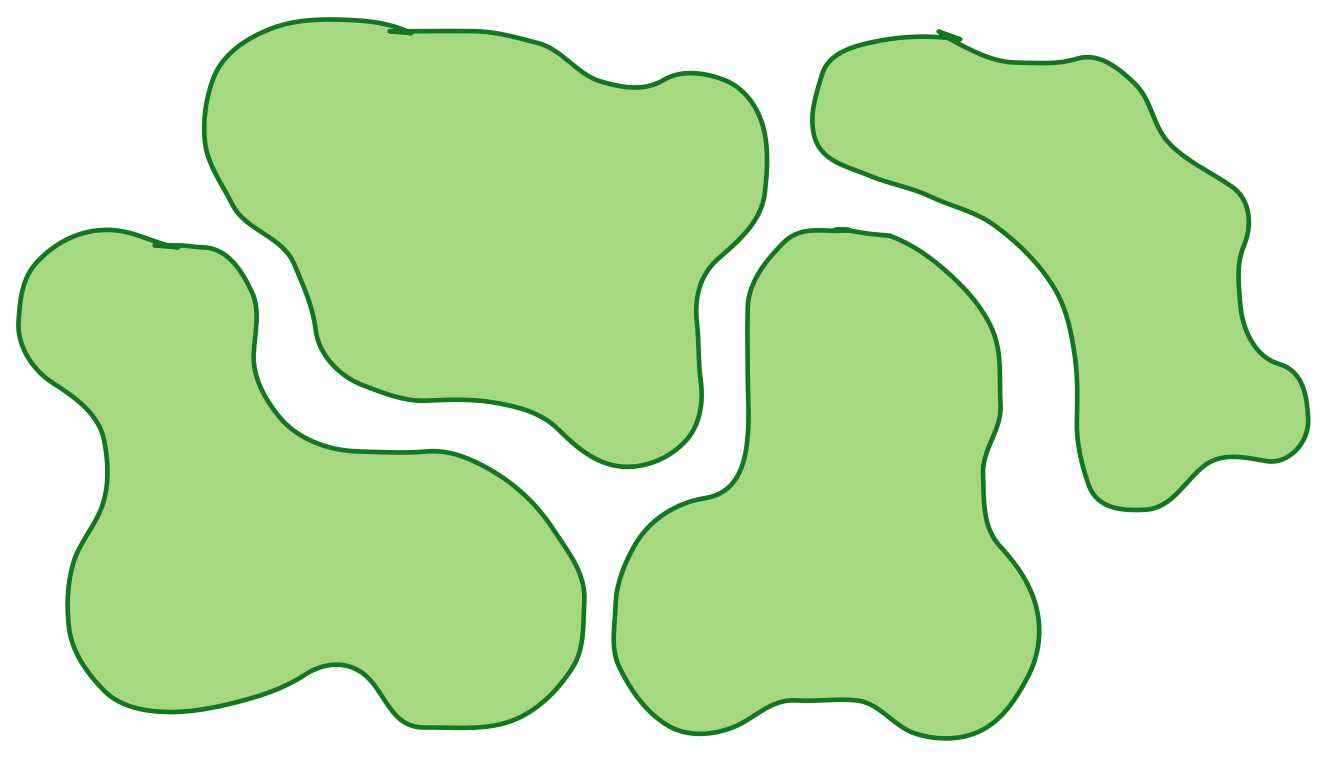
\includegraphics[width=2cm]{images/intro/objective_geom.png}};
						\node[title,font=\Large] at (1.6,0.1) {+};
						\node at (3.5,0.8) {Several Functions};
						\node[draw=none, inner sep=0pt] at (3.5,0) {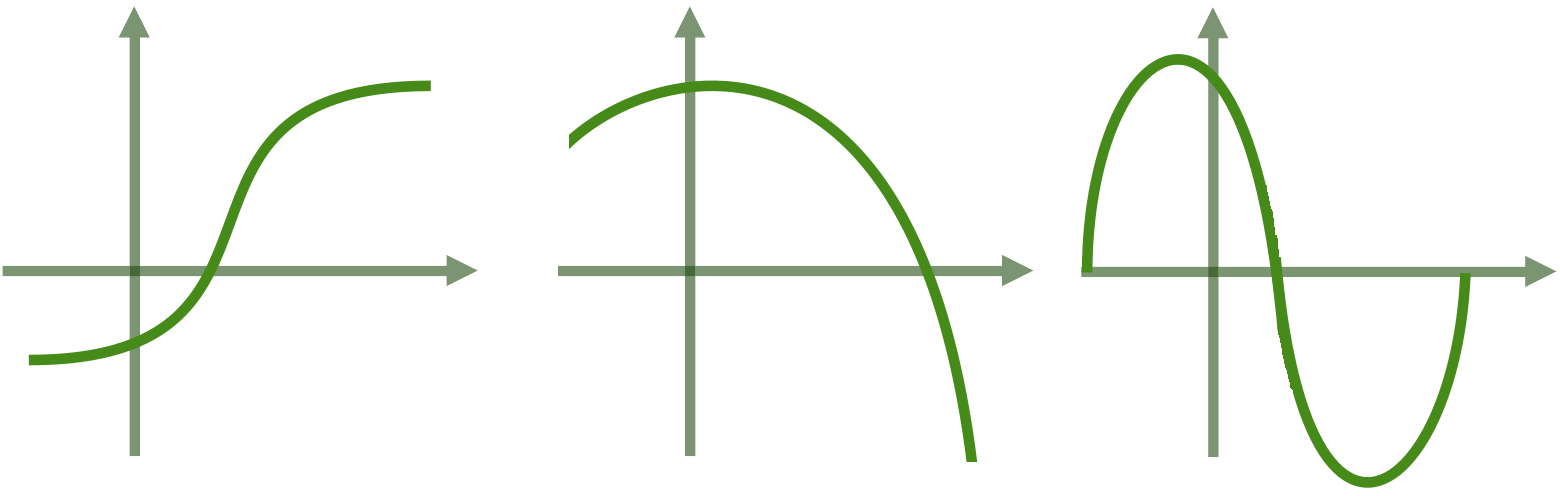
\includegraphics[width=3cm]{images/intro/objective_fct.png}};
						
						% Ajouter une flèche entre les deux rectangles
						\draw[->, title, line width=1.5pt] (5.5,0.1) -- (6.5,0.1);
						%		
						\node at (8,0.8) {Train a PINNs};
						\node[draw=none, inner sep=0pt] at (8,-0.1) {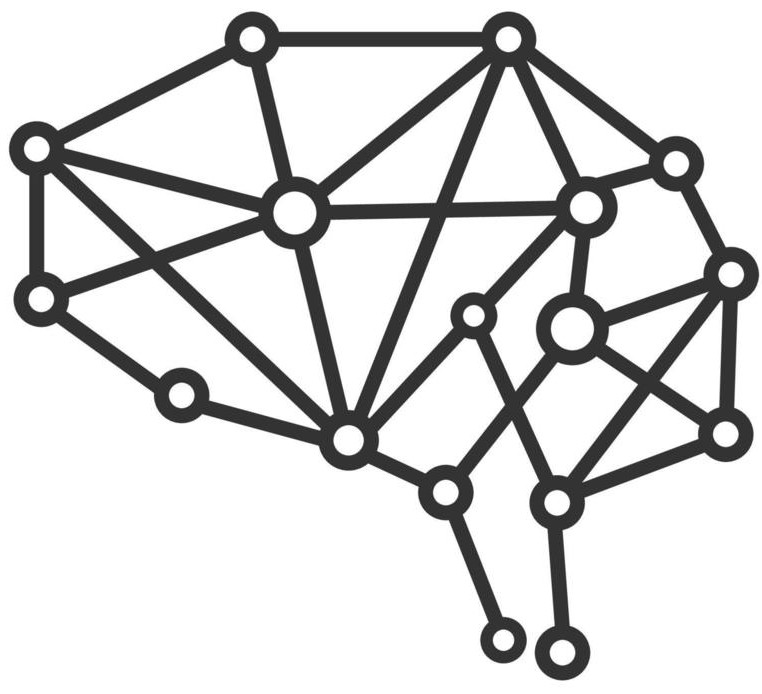
\includegraphics[width=1.5cm]{images/intro/objective_pinns.jpg}};				
					\end{tikzpicture}
				}%
			\end{figure}
			
			\textbf{ONLINE :}
			
			\vspace{-25pt}
			
			\begin{figure}[htb]
				\centering
				\resizebox{\textwidth}{!}{%
					\begin{tikzpicture}
						\node at (0,0.8) {1 Geometry - 1 Function};
						\node[draw=none, inner sep=0pt] at (0,0) {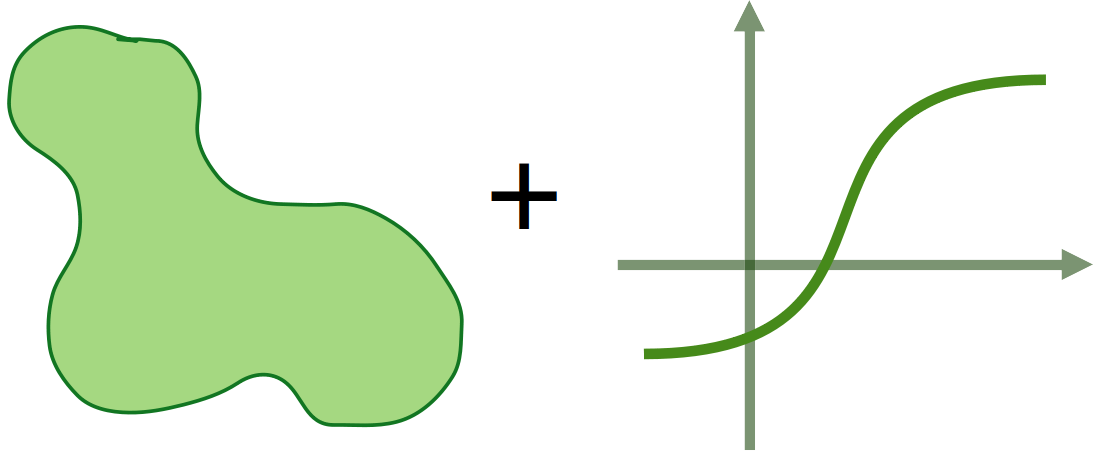
\includegraphics[width=2cm]{images/intro/objective_onegeom_onefct.png}};
						%		\node[title,font=\Large] at (1.6,0.1) {+};
						%		\node at (3.5,0.8) {Several Functions};
						%		\node[draw=none, inner sep=0pt] at (3.5,0) {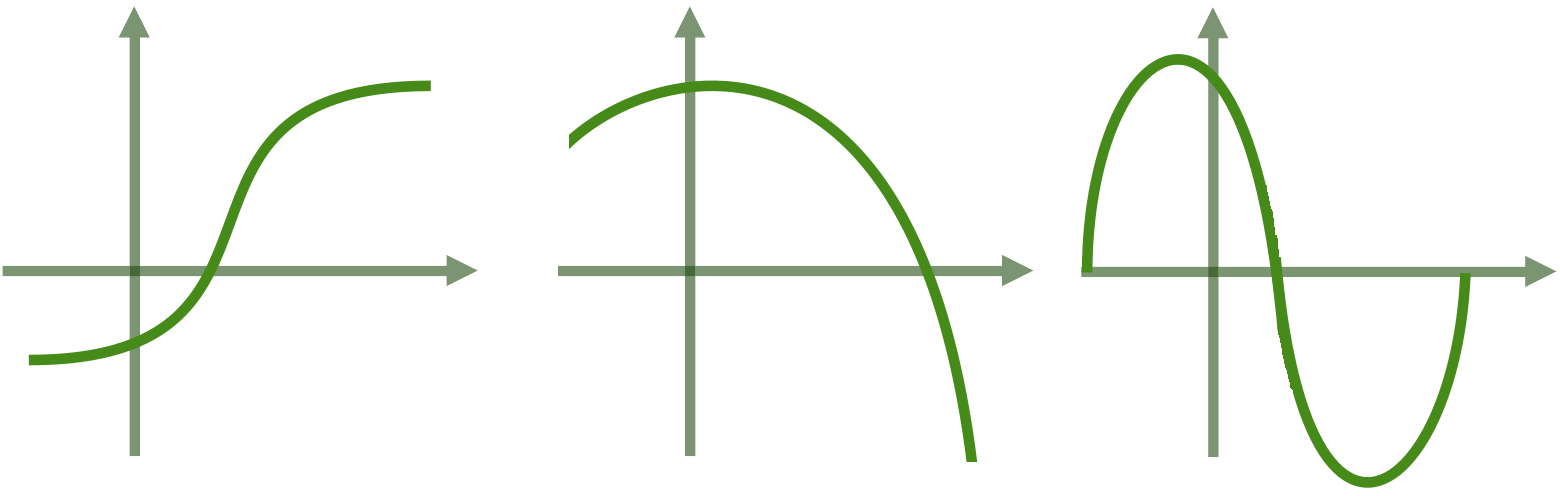
\includegraphics[width=3cm]{images/intro/objective_fct.png}};
						
						\draw[->, title, line width=1.5pt] (2,0.1) -- (3,0.1);
						
						\node[align=center] at (4,1) {Get PINNs \\ prediction};
						\node[draw=none, inner sep=0pt] at (4,-0.1) {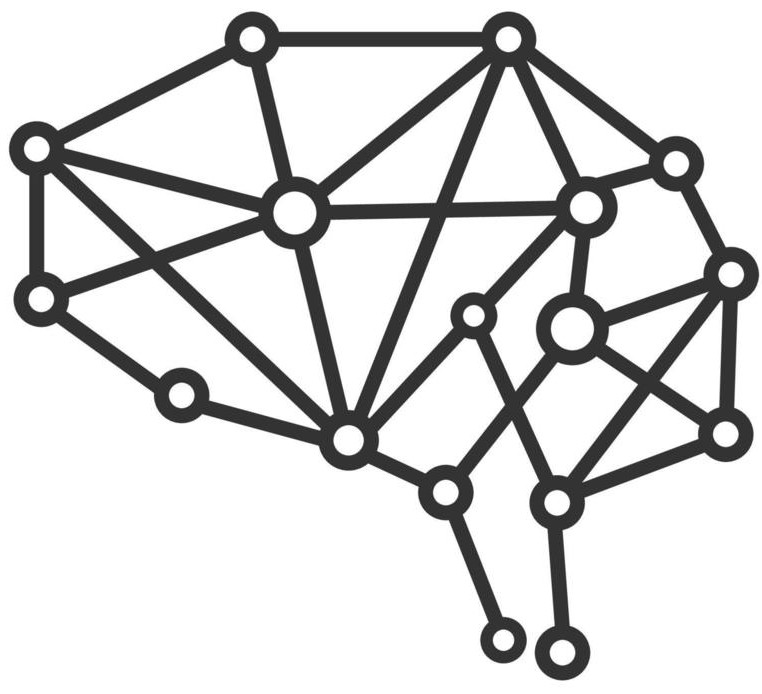
\includegraphics[width=1.5cm]{images/intro/objective_pinns.jpg}};
						
						% Ajouter une flèche entre les deux rectangles
						\draw[->, title, line width=1.5pt] (5.5,0.1) -- (6.5,0.1);
						%		
						\node[align=center] at (8,1) {Correct prediction \\ with $\phi$-FEM};
						\node[draw=none, inner sep=0pt] at (8,-0.1) {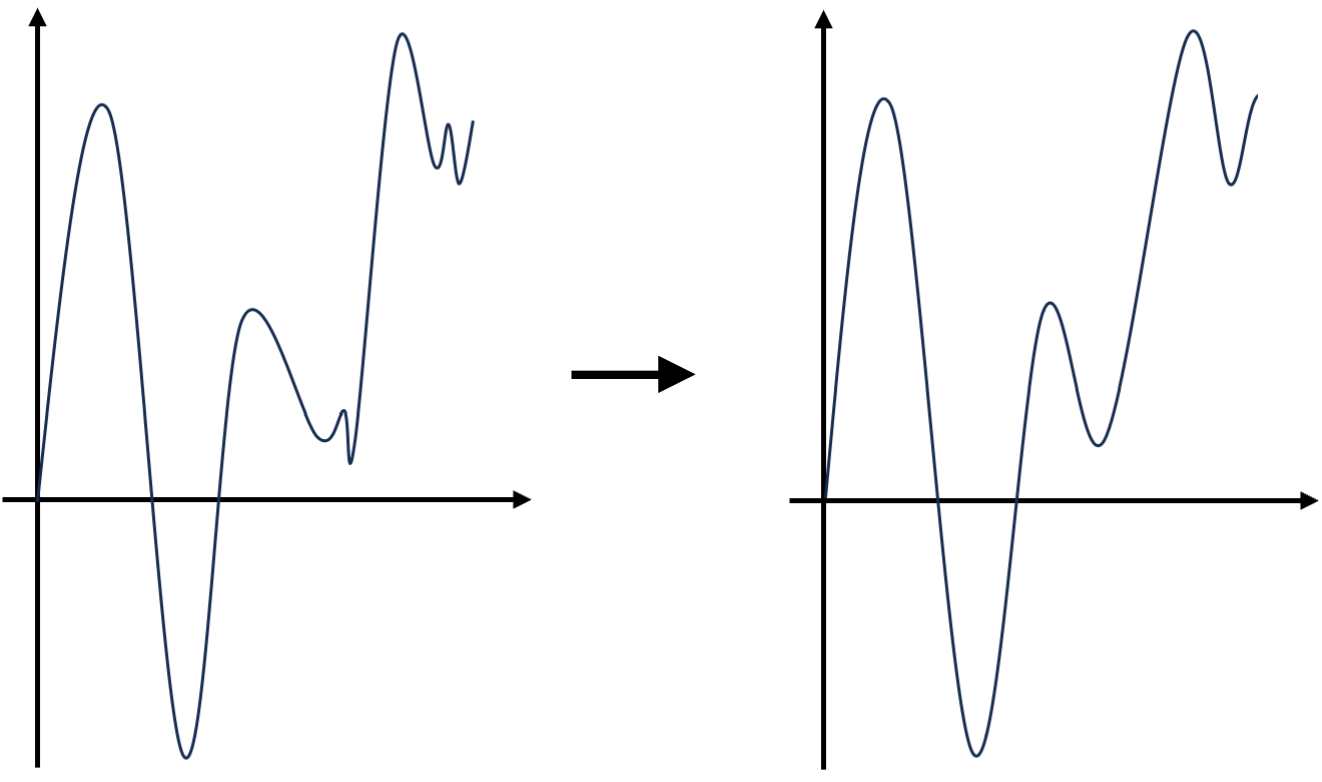
\includegraphics[width=2.5cm]{images/intro/objective_corr.png}};		
					\end{tikzpicture}
				}%
			\end{figure}
		\end{tcolorbox}
	\end{center}

    \textbf{Evolution :}

    \small
    % \setstretch{0.5}
    \begin{itemize}
        \item Geometry : 2D, simple, fixed (as circle, ellipse..) $ \; \rightarrow \;$ 3D / complex / variable
        \item PDE : simple, static (Poisson problem) $\; \rightarrow \;$ complex / dynamic (elasticity, hyper-elasticity)
        \item Neural Network : simple and defined everywhere (PINNs) $\; \rightarrow \;$ Neural Operator
    \end{itemize}
\end{frame}

\begin{frame}{Problem considered}
    \textbf{Elliptic problem with Dirichlet conditions :} \\
    Find $u : \Omega \rightarrow \mathbb{R}^d (d=1,2,3)$ such that
    \begin{equation}
    	\left\{\begin{aligned}
    		&L(u)=-\nabla \cdot (A(x) \nabla u(x)) + c(x)u(x) = f(x) \quad \text{in } \Omega, \\
    		&u(x) = g(x) \quad \text{on } \partial \Omega
    	\end{aligned}\right. \label{edp}
    \end{equation}
	with $A$ a definite positive coercivity condition and $c$ a scalar. We consider $\Delta$ the Laplace operator, $\Omega$ a smooth bounded open set and $\Gamma$ its boundary. 
    
    \textbf{Weak formulation :}
    \begin{equation*}
    	\text{Find } u\in V \text{ such that } a(u, v) = l (v) \forall v\in V
    \end{equation*}
    
    with
    \begin{align*}
    	a(u,v)&=\int_{\Omega} (A(x)\nabla u(x)) \cdot \nabla v(x) + c(x)u(x)v(x) \, dx \\
    	l(v)&=\int_{\Omega} f(x)v(x) \, dx
    \end{align*}
    
    \footnotesize
    \textit{Remark :} For simplicity, we will not consider 1st order terms. 

%    We will define by
%    \begin{equation*}
%        ||u_{ex}-u_{method}||_{0,\Omega}^{(rel)}=\frac{\int_\Omega (u_{ex}-u_{method})^2}{\int_\Omega u_{ex}^2}
%    \end{equation*}
%    the relative error between
%    \begin{itemize}
%        \item $u_{ex}$ : the exact solution  
%        \item $u_{method}$ : the solution obtained by a method \\
%        (can be : FEM or $\phi$-FEM, a correction solver or the prediction of an neural network).
%    \end{itemize}
\end{frame}

\begin{frame}{Numerical methods}
	\textbf{Objective :} Show that the philosophy behind most ofd the methods are the same.
	\begin{center}
		Mesh-based methods \hspace{5pt} // \hspace{5pt} Physically informed learning
	\end{center}
	
	\textbf{Numerical methods :} Discrete an infinite-dimensional problem (unknown = function) and solve it in a finite-dimensional space (unknown = vector).
	\begin{enumerate}[\textbullet]
		\item \textbf{Encoding :} we encode the problem in a finite-dimensional space
		\item \textbf{Approximation :} solve the problem in finite-dimensional space
		\item \textbf{Decoding :} bring the solution back into infinite dimensional space
	\end{enumerate}
	
	\begin{center}
		\begin{tabular}{|c|c|c|}
			\hline
			\textbf{Encoding} & \textbf{Approximation} & \textbf{Decoding} \\
			\hline
			$f \; \rightarrow \theta_f$ & $\theta_f \; \rightarrow \theta_u$ & $\theta_u \; \rightarrow u_\theta$ \\
			\hline
		\end{tabular}
	\end{center}
\end{frame}

	
	
	\renewcommand{\insertsectionheadSubtitle}{This section is based on \citep{ours_2025}.}
	\section{Enriched finite element method using PINNs}
	\subsection{Additive approach}

\begin{frame}{Additive approach}
	\textbf{Variational Problem :} Let $u_{\theta} \in H^{k+1}(\Omega)\cap H^1_0(\Omega)$.
	
	\vspace{-5pt}
	\begin{equation}
		\label{eq:weakplus}
		\text{Find } p_h^+ \in V_h^0 \text{ such that}, \forall v_h \in V_h^0, a(p_h^+,v_h) = l(v_h) - a(u_{\theta},v_h),\tag{$\mathcal{P}_h^+$}
	\end{equation}
	
	\vspace{5pt}
	\begin{minipage}[t]{0.6\linewidth}
		with the \textcolor{red}{enriched trial space $V_h^+$} defined by
		\begin{equation*}
			V_h^+ = \left\{
			u_h^+= u_{\theta} + p_h^+, \quad p_h^+ \in V_h^0
			\right\}.
		\end{equation*}
	
		\vspace{20pt}
	
		\textbf{General Dirichlet BC :} If $u=g$ on $\partial \Omega$, then
		\[
			p_h^+ = g - u_{\theta} \text{\quad on } \partial \Omega,
		\]
		with $u_\theta$ the PINN prior. 
	\end{minipage} \qquad \begin{minipage}[t][][b]{0.28\linewidth}
		\vspace{-15pt}
		\centering
		\pgfimage[width=\linewidth]{images/correction/correction.pdf}
	\end{minipage}
\end{frame}

\begin{frame}{Convergence analysis}
	\vspace{-10pt}
	\hypersetup{
		citecolor=white,
	}

	\begin{mytheo}{Convergence analysis of the standard FEM \footnotesize\citep{Ern2004TheoryAP}\normalsize}{fem}
		We denote $u_h\in V_h$ the solution of \eqref{eq:weakform} with $V_h$ the standard trial space. Then,
		\vspace{-5pt}
		\begin{equation*}
			| u-u_h|_{H^1} \leqslant C_{H^1} \, h^{k} |u|_{H^{k+1}},
		\end{equation*}
		\begin{equation*}
			\| u-u_h\|_{L^2} \leqslant C_{L^2} \, h^{k+1} |u|_{H^{k+1}}.
		\end{equation*}
	\end{mytheo}
	
	\begin{mytheo}{Convergence analysis of the enriched FEM \footnotesize\citep{ours_2025}\normalsize}{add}
		We denote $u_h^+\in V_h^+$ the solution of \eqref{eq:weakplus} with $V_h^+$ the enriched trial space. Then,
		\vspace{-5pt}
		\begin{equation*}
			| u-u_h^+|_{H^1} \leqslant \fcolorbox{orange}{other!10!white}{$\frac{| u-u_{\theta} |_{H^{k+1}}}{| u |_{H^{k+1}}}$} \left(C_{H^1} \, h^{k} |u|_{H^{k+1}}\right),
		\end{equation*}
		\begin{equation*}
			\| u-u_h^+\|_{L^2} \leqslant \fcolorbox{orange}{other!10!white}{$\frac{| u-u_{\theta} |_{H^{k+1}}}{| u |_{H^{k+1}}}$} \left(C_{L^2} \, h^{k+1} |u|_{H^{k+1}}\right).
		\end{equation*}
	\end{mytheo}

	\hypersetup{
		citecolor=other,
	}

	\footnotesize
	\textcolor{orange}{Gains of the additive approach.}
\end{frame}

\subsection{Numerical results \filledstar}

\begin{frame}{1st problem considered} 
	\textbf{Problem statement:} Considering an \textcolor{red}{Anisotropic Elliptic problem with Dirichlet BC}:
	\vspace{-5pt}
	\begin{equation*}
		\left\{
		\begin{aligned}
			-\text{div}(D\nabla u) & = f, \; &  & \text{in } \; \Omega, \\
			u         & =0, \;  &  & \text{on } \; \partial\Omega,
		\end{aligned}
		\right.
		% \label{eq:Ell2D}\tag{$\mathcal{P}$}
	\end{equation*}

	with $\Omega=[0,1]^2$ and $\mathcal{M}=[0.4, 0.6]\times [0.4, 0.6]\times [0.01,1]\times [0.1,0.8]$ ($p=4$).
	
	\vspace{8pt}
	\textbf{Right-hand side :}

	\vspace{-5pt}
	\begin{equation*}
		f(\bm{x},\bm{\mu})=\exp\left(-\frac{(x-\mu_1)^2+(y-\mu_2)^2}{0.025\sigma^2}\right).
	\end{equation*}
	
	\textbf{Diffusion matrix :} (symmetric and positive definite)
	\begin{equation*}
		D(\bm{x},\bm{\mu})=\begin{pmatrix}
			\epsilon x^2+y^2 & (\epsilon-1)xy \\
			(\epsilon-1)xy & x^2+\epsilon y^2
		\end{pmatrix}.
	\end{equation*}

	\vspace{2pt}
	\small
	\textbf{PINN training:} Imposing BC exactly with a level-set function.
\end{frame}

\begin{frame}{Numerical results}
	\hspace{-5pt}\begin{minipage}[t]{0.46\linewidth}
		\textbf{Error estimates :} 1 set of parameters.
		$$\bm{\mu}^{(1)}=(0.51,0.54,0.52,0.55)$$
		\vspace{-35pt}
		\begin{figure}[H]
			\cvgFEMCorrAlldeg{images/numeric/elliptic/cvg/FEM_case3_v1_param1.csv}{images/numeric/elliptic/cvg/Corr_case3_v1_param1.csv}{1e-9}
		\end{figure}
	\end{minipage} \qquad \small
	\begin{minipage}[t]{0.48\linewidth}
	\end{minipage}
\end{frame}

\begin{frame}[noframenumbering]{Numerical results}
	\hspace{-5pt}\begin{minipage}[t]{0.46\linewidth}
		\textbf{Error estimates :} 1 set of parameters.
		$$\bm{\mu}^{(1)}=(0.51,0.54,0.52,0.55)$$
		\vspace{-35pt}
		\begin{figure}[H]
			\cvgFEMCorrAlldeg{images/numeric/elliptic/cvg/FEM_case3_v1_param1.csv}{images/numeric/elliptic/cvg/Corr_case3_v1_param1.csv}{1e-9}
		\end{figure}
	\end{minipage} \qquad \small
	\begin{minipage}[t]{0.48\linewidth}
		\textbf{Gains achieved :} $n_p=50$ sets of parameters.
		$$\mathcal{S}=\left\{\bm{\mu}^{(1)},\dots,\bm{\mu}^{(n_p)}\right\}$$
		\vspace{-15pt}
		\begin{table}[H]
			\gainstableallq{images/numeric/elliptic/gains/Tab_stats_case3_v1.csv}
		\end{table}

		\normalsize\centering\vspace{-20pt}
		$$N=20$$

		\vspace{-5pt}
		Gain : $\| u-u_h\|_{L^2} / \| u-u_h^+\|_{L^2}$ \\
		
		\small\vspace{8pt}
		Cartesian mesh : $N^2$ nodes.
	\end{minipage}
\end{frame}

\begin{frame}{Numerical solutions}
	\begin{figure}[!ht] \centering
		\includegraphics[width=0.33\linewidth]{images/numeric/elliptic/plots/standalone_solutions_cropped.pdf}		
		\includegraphics[width=0.7\linewidth]{images/numeric/elliptic/plots/standalone_errors.pdf}
	\end{figure}

	\vspace{-8pt}
	$$\bm{\mu}^{(2)}=(0.46,0.52,0.05,0.12)$$
\end{frame}

\begin{frame}{2nd problem considered} 
	\textbf{Problem statement:} Considering the \textcolor{red}{Poisson problem with mixed BC}:
	\vspace{-5pt}
	\begin{equation*}
		\left\{
		\begin{aligned}
			-\Delta u & = f, \; &  & \text{in } \; \Omega \times \mathcal{M}, \\
			u         & = g, \;  &  & \text{on } \; \Gamma_E \times \mathcal{M}, \\
			\smash{\frac{\partial u}{\partial n}}+u  & = g_R, \;  &  & \text{on } \; \Gamma_I \times \mathcal{M},
		\end{aligned}
		\right.
		% \label{eq:Lap2DMixed}\tag{$\mathcal{P}$}
	\end{equation*}

	with $\Omega=\{(x,y)\in\mathbb{R}^2, \; 0.25\le x^2+y^2\le 1\}$ and $\mathcal{M}=[2.4,2.6]$ ($p=1$).
		
	\vspace{8pt}
	\textbf{Analytical solution :}

	\vspace{-12pt}
	\begin{equation*}
		% \label{eq:analytical_solution_Lap2D}
		u(\bm{x};\bm{\mu})= 1 - \frac{\ln\big(\mu_1\sqrt{x^2+y^2}\big)}{\ln(4)},
	\end{equation*}
	\vspace{-5pt}
	
	\textbf{Boundary conditions :}
	\begin{equation*}
		g(\bm{x};\bm{\mu})=1 - \frac{\ln(\mu_1)}{\ln(4)} \quad \text{and} \quad g_R(\bm{x};\bm{\mu})=2 + \frac{4-\ln(\mu_1)}{\ln(4)}.
	\end{equation*}

	\vspace{2pt}
	\small
	\textbf{PINN training:} Imposing mixed BC exactly in the PINN\footcite{Sukumar_2022}.

	\vspace{8pt}
\end{frame}

\begin{frame}{Numerical results}
	\hspace{-5pt}\begin{minipage}[t]{0.46\linewidth}
		\textbf{Error estimates :} 1 set of parameters.
		$$\bm{\mu}^{(1)}=2.51$$
		\vspace{-35pt}
		\begin{figure}[H]
			\cvgFEMCorrAlldeg{images/numeric/poisson/mixed/cvg/FEM_case5_v2_param1.csv}{images/numeric/poisson/mixed/cvg/Corr_case5_v2_param1.csv}{1e-10}
		\end{figure}
	\end{minipage} \qquad \small
	\begin{minipage}[t]{0.48\linewidth}
		\textbf{Gains achieved :} $n_p=50$ sets of parameters.
		$$\mathcal{S}=\left\{\bm{\mu}^{(1)},\dots,\bm{\mu}^{(n_p)}\right\}$$
		\vspace{-15pt}
		\begin{table}[H]
			\gainstableallq{images/numeric/poisson/mixed/gains/Tab_stats_case5_v2.csv}
		\end{table}

		\normalsize\centering\vspace{-20pt}
		$$h=1.33\cdot 10^{-1}$$

		\vspace{-5pt}
		Gain : $\| u-u_h\|_{L^2} / \| u-u_h^+\|_{L^2}$ \\
		\end{minipage}
\end{frame}

\begin{frame}{Numerical solutions}
	\begin{figure}[!ht] \centering
		\includegraphics[width=0.31\linewidth]{images/numeric/poisson/mixed/plots/standalone_solutions_cropped.pdf}
		\includegraphics[width=0.7\linewidth]{images/numeric/poisson/mixed/plots/standalone_errors.pdf}
	\end{figure}

	\vspace{-8pt}
	$$\bm{\mu}^{(1)}=2.51 $$
\end{frame}
	\renewcommand{\insertsectionheadSubtitle}{}

	\section{New lines of research}
	\subsection{Complex geometries}

\begin{frame}{Learn a regular levelset}		
    \vspace{-10pt}
    \hypersetup{
		citecolor=white,
	}

    \begin{mytheo}{\footnotesize\citep{clemot_neural_2023}\normalsize}{fem}
		If we have a boundary domain $\Gamma$, the SDF is solution to the Eikonal equation:
		
		\begin{minipage}{0.7\linewidth}
			\hspace{100pt}
			$\left\{\begin{aligned}
				&||\nabla\phi(X)||=1, \; X\in\mathcal{O} \\
				&\phi(X)=0, \; X\in\Gamma \\
				&\nabla\phi(X)=n, \; X\in\Gamma
			\end{aligned}\right.$
		\end{minipage}
		\begin{minipage}{0.25\linewidth}
			\centering
			\pgfimage[width=0.7\linewidth]{images/newlines/levelset/points_normals.png}
		\end{minipage}
		
		with $\mathcal{O}$ a box which contains $\Omega$ completely and $n$ the exterior normal to $\Gamma$.
	\end{mytheo}

    \hypersetup{
        citecolor=other,
    }

    \vspace{5pt}

    \textbf{Objective:} Move on to complex geometries by using a levelset function to

    \begin{itemize}
        \item Sample points in the domain $\Omega$ for the PINN training.
        \item Impose exactly the boundary condition in PINN \citep{Sukumar_2022}.
    \end{itemize}

    \vspace{5pt}

	\textbf{How to learn a regular levelset ?} with a PINN by \textcolor{orange}{adding a regularization term},
	\vspace{-5pt}
	\begin{equation*}
		J_{reg} = \int_\mathcal{O} |\Delta\phi|^2,
	\end{equation*}
    and a sample of boundary points that considers the \textcolor{orange}{curvature} of $ \Gamma$. \filledstar

    % Curvature
\end{frame}

\begin{frame}{Numerical results}		
    \begin{figure}[!ht] \centering
		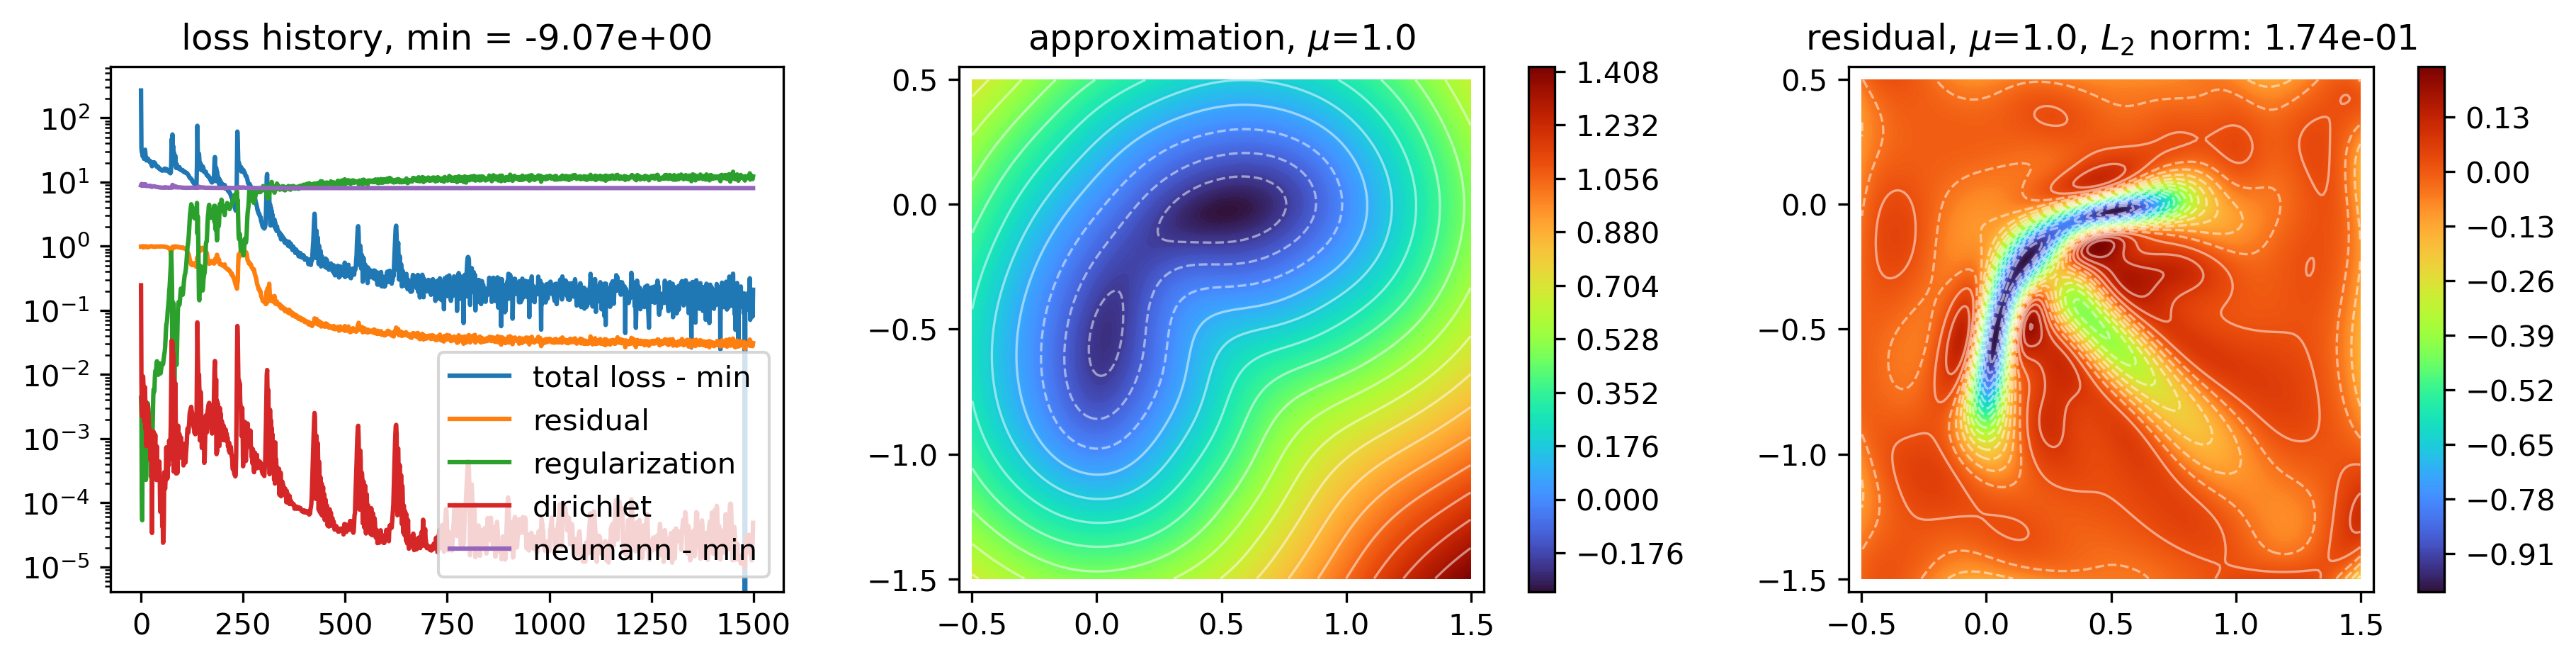
\includegraphics[width=\linewidth]{images/newlines/levelset/EikonalBean_curvature.png}

        % \vspace{10pt}

		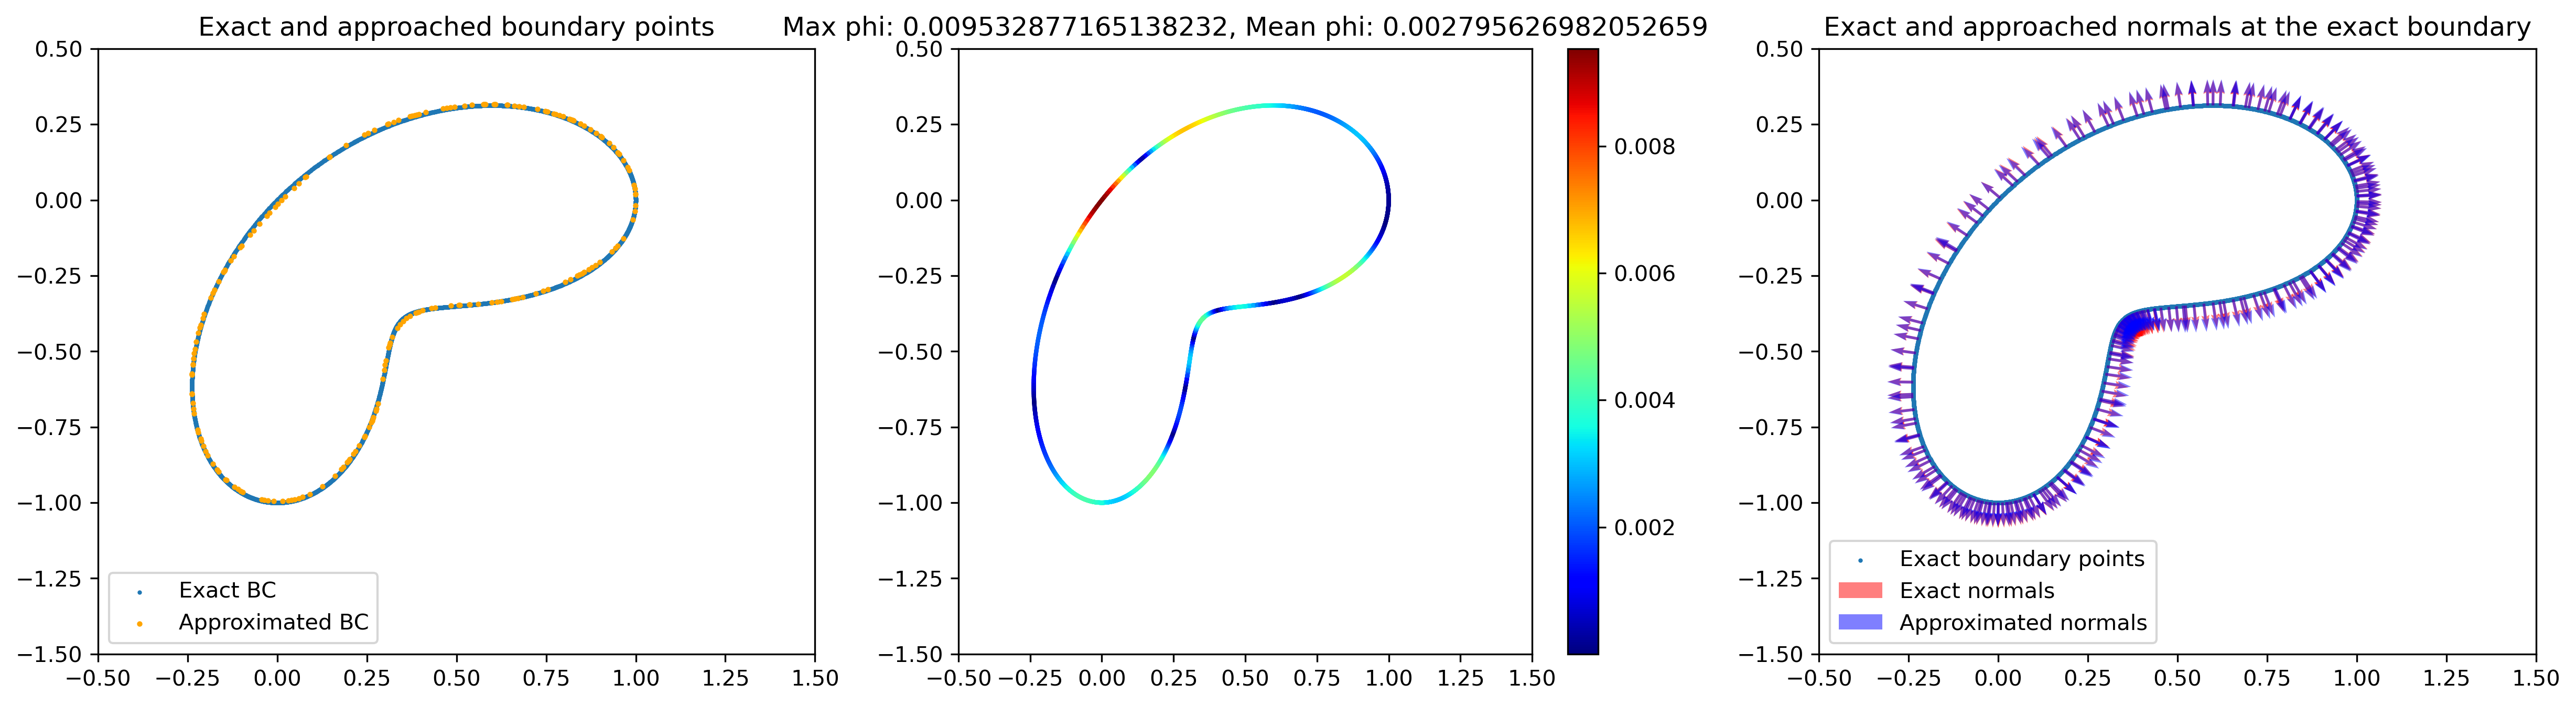
\includegraphics[width=\linewidth]{images/newlines/levelset/boundary_curvature.png}
	\end{figure}

    % \vspace{-5pt}
    % TODO : Ajouter résultats "Poisson on Bean" + Mettre au propre les images. 
\end{frame}

\subsection{\filledstar A posteriori error estimates}

\begin{frame}{Problem considered} 
	\textbf{Problem statement:} Considering the \textcolor{red}{Poisson problem with Dirichlet BC}:
	\vspace{-5pt}
	\begin{equation*}
		\left\{
		\begin{aligned}
			-\Delta u & = f, \; &  & \text{in } \; \Omega \times \mathcal{M}, \\
			u         & = 0, \;  &  & \text{on } \; \Gamma \times \mathcal{M},
		\end{aligned}
		\right.
		% \label{eq:Lap2DMixed}\tag{$\mathcal{P}$}
	\end{equation*}

	with $\Omega=[-0.5\pi,0.5\pi]^2$ and $\mathcal{M}=[-0.5,0.5]^2$ ($p=2$).
	
	\vspace{2pt}
	\textbf{Analytical solution :}

	\vspace{-12pt}
	\begin{equation*}
		% \label{eq:analytical_solution_Lap2D}
		u(\bm{x};\bm{\mu})= \exp\left(-\frac{(x-\mu_1)^2+(y-\mu_2)^2}{2(0.15)^2}\right)\sin(2x)\sin(2y).
	\end{equation*}

	\vspace{2pt}
	\small
	\textbf{PINN training:} Imposing Dirichlet BC exactly in the PINN.

	\vspace{8pt}
\end{frame}

\begin{frame}{Adaptive mesh refinement}	
    \textbf{Adaptive refinement loop} using Dorfler marking strategy. \refappendix{frame:amr} %(residual estimator)
    
    \begin{center}
        \textbf{Standard FEM}
        \vspace{2pt}

        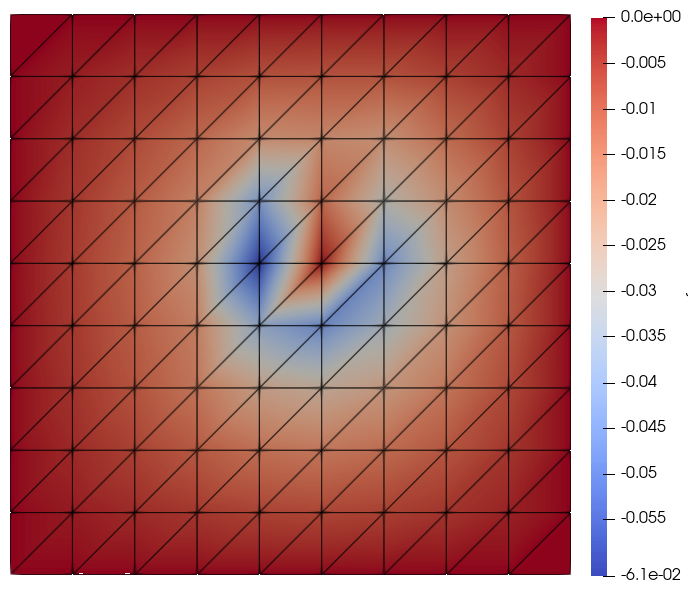
\includegraphics[width=0.2\linewidth]{images/newlines/mesh/explications/fem/u_h.png}
        \quad
        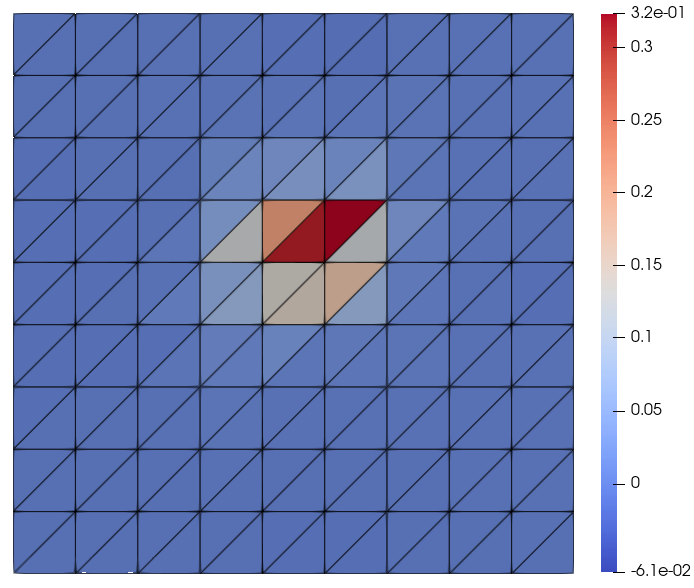
\includegraphics[width=0.2\linewidth]{images/newlines/mesh/explications/fem/eta_h.png}
        \quad
        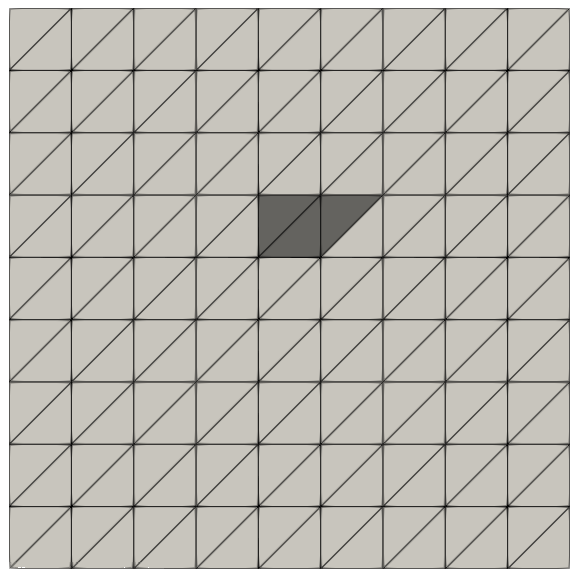
\includegraphics[width=0.17\linewidth]{images/newlines/mesh/explications/fem/marking.png}
        \qquad
        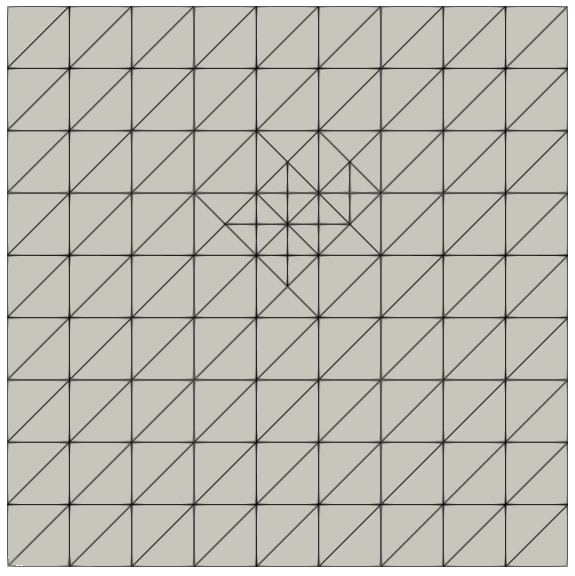
\includegraphics[width=0.17\linewidth]{images/newlines/mesh/explications/fem/refined.png}
    \end{center}

    \vspace{-10pt}
    $\cdots\hspace{1pt}\longrightarrow\hspace{8pt}
    \text{SOLVE}\hspace{18pt}\longrightarrow\hspace{6pt}
    \text{ESTIMATE}\hspace{8pt}\longrightarrow\hspace{14pt}
    \text{MARK}\hspace{14pt}\longrightarrow\hspace{8pt}
    \text{REFINE}\hspace{4pt}\longrightarrow\hspace{1pt}
    \cdots$

    \hspace{45pt}$\text{on }u_h\hspace{55pt}\eta_{res,T}$

    \vspace{8pt}
    \textbf{Local residual estimator (in $L^2$ norm):} Let $T$ be a cell of $\mathcal{T}_h$ .

    \vspace{-8pt}
    % $$\eta_{res,T}^2 = h_T^4 \|\Delta u_h + f_h\|_{L^2(T)}^2 + \frac{1}{2} \sum_{E \in \partial T} h_E^2 \|[\nabla u_h\cdot n]\|_{L^2(E)}^2$$
    $$\eta_{res,T}^2 = h_T^2 \|\Delta u_h + f_h\|_{L^2(T)}^2 + \frac{1}{2} \sum_{E \in \partial T} h_E \|[\nabla u_h\cdot n]\|_{L^2(E)}^2$$
    with $h_\bullet$ the size of $\bullet$ and considering the Poisson problem.

    % Considering the Poisson problem with Dirichlet boundary conditions.

    % (en précisant que c'est le coût du solve qui est le plus important)
\end{frame}

\begin{frame}[noframenumbering]{Adaptive mesh refinement}	
    \textbf{Adaptive refinement loop} using Dorfler marking strategy.
    
    \begin{center}
        \textcolor{red}{\textbf{Additive Approach}}
        \vspace{2pt}

        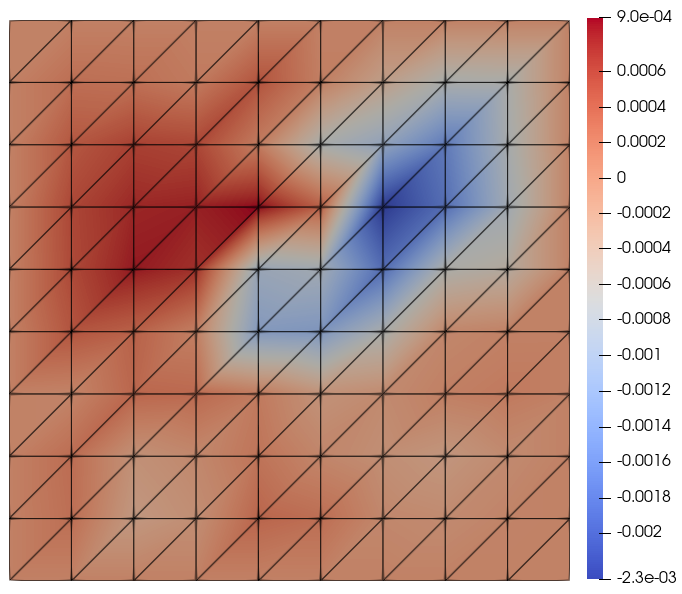
\includegraphics[width=0.2\linewidth]{images/newlines/mesh/explications/add/p_h.png}
        \quad
        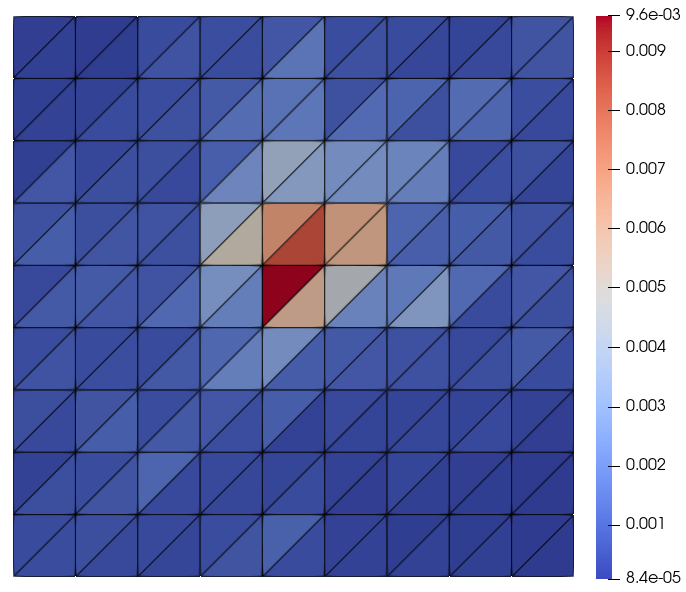
\includegraphics[width=0.2\linewidth]{images/newlines/mesh/explications/add/eta_h_add.png}
        \quad
        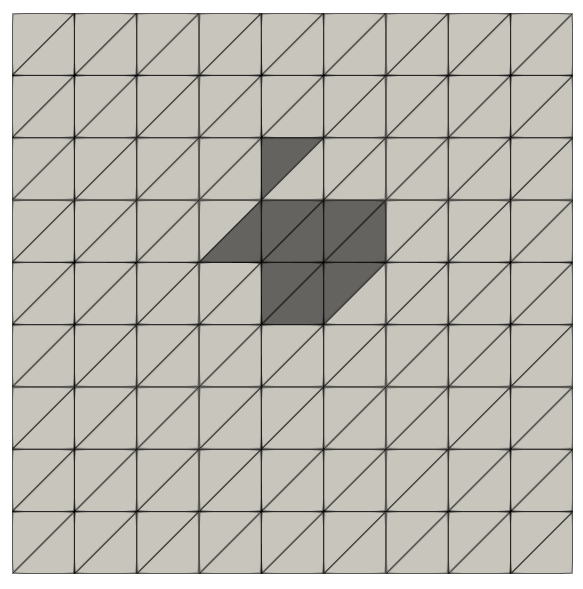
\includegraphics[width=0.17\linewidth]{images/newlines/mesh/explications/add/marking_add.png}
        \qquad
        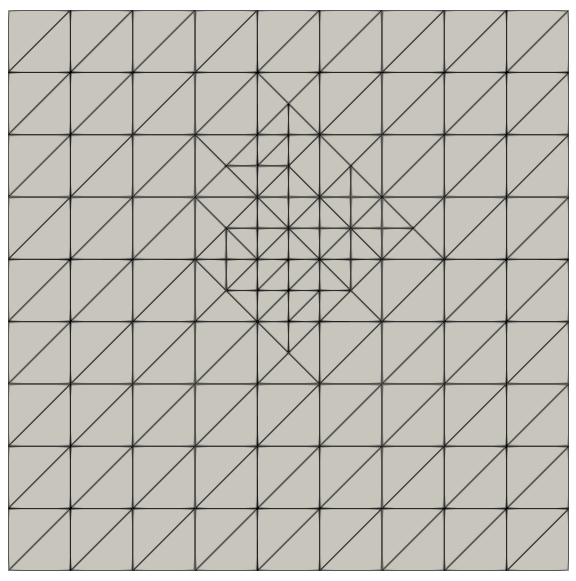
\includegraphics[width=0.17\linewidth]{images/newlines/mesh/explications/add/refined_add.png}
    \end{center}

    \vspace{-10pt}
    $\cdots\hspace{1pt}\longrightarrow\hspace{8pt}
    \text{SOLVE}\hspace{18pt}\longrightarrow\hspace{6pt}
    \text{ESTIMATE}\hspace{8pt}\longrightarrow\hspace{14pt}
    \text{MARK}\hspace{14pt}\longrightarrow\hspace{8pt}
    \text{REFINE}\hspace{4pt}\longrightarrow\hspace{1pt}
    \cdots$

    \hspace{45pt}$\text{on }\textcolor{red}{p_h^+}\hspace{55pt}\eta_{res,T}$

    \vspace{8pt}
    \textbf{Local residual estimator (in $L^2$ norm):} Let $T$ be a cell of $\mathcal{T}_h$ .

    \vspace{-8pt}
    % $$\eta_{res,T}^2 = h_T^4 \|\textcolor{red}{\big((\Delta u_\theta)_h + \Delta p_h^+\big) + f_h}\|_{L^2(T)}^2 + \frac{1}{2} \sum_{E \in \partial T} h_E^2 \|\textcolor{red}{[\nabla p_h^+\cdot n]}\|_{L^2(E)}^2$$
    $$\eta_{res,T}^2 = h_T^2 \|\textcolor{red}{\big((\Delta u_\theta)_h + \Delta p_h^+\big) + f_h}\|_{L^2(T)}^2 + \frac{1}{2} \sum_{E \in \partial T} h_E \|\textcolor{red}{[\nabla p_h^+\cdot n]}\|_{L^2(E)}^2$$
    with $h_\bullet$ the size of $\bullet$ and considering the Poisson problem.
\end{frame}

\begin{frame}[noframenumbering]{Adaptive mesh refinement}	
    \textbf{Adaptive refinement loop} using Dorfler marking strategy.
    
    \begin{center}
        \textbf{Additive Approach \textcolor{red}{- No resolution}}
        \vspace{2pt}

        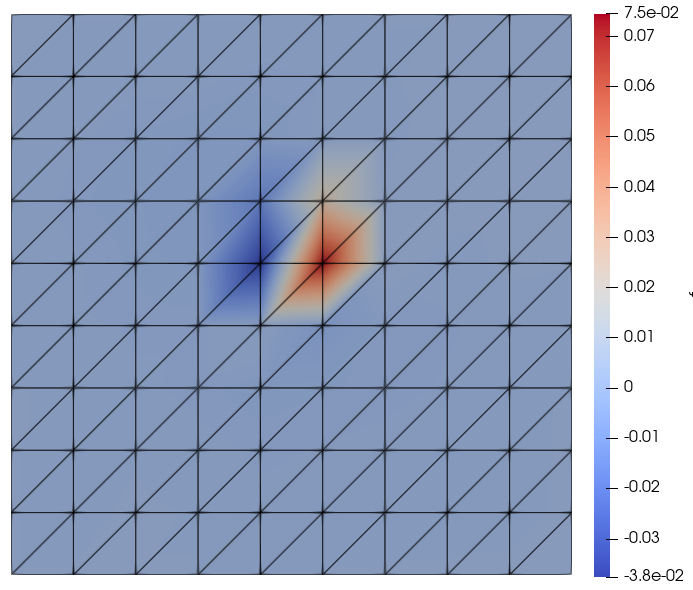
\includegraphics[width=0.2\linewidth]{images/newlines/mesh/explications/addnet/u_theta_h.png}
        \quad
        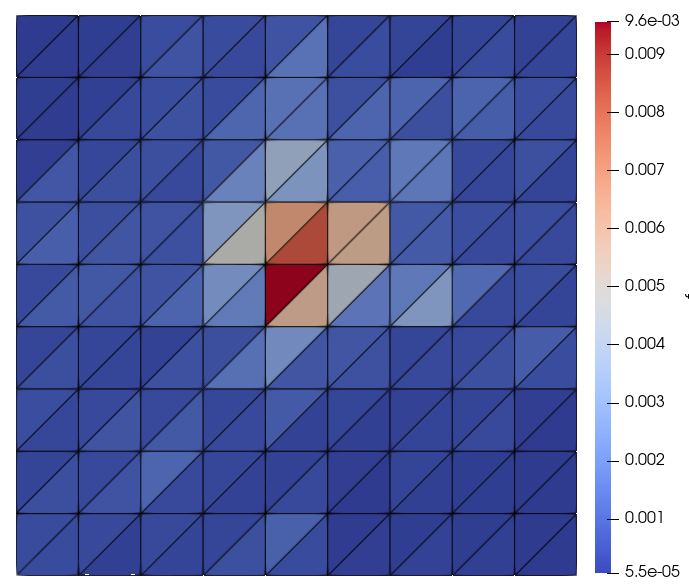
\includegraphics[width=0.2\linewidth]{images/newlines/mesh/explications/addnet/eta_h_addnet.png}
        \quad
        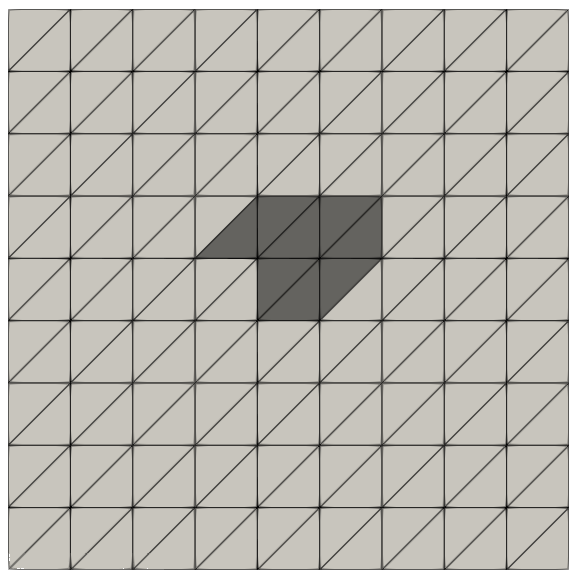
\includegraphics[width=0.17\linewidth]{images/newlines/mesh/explications/addnet/marking_addnet.png}
        \qquad
        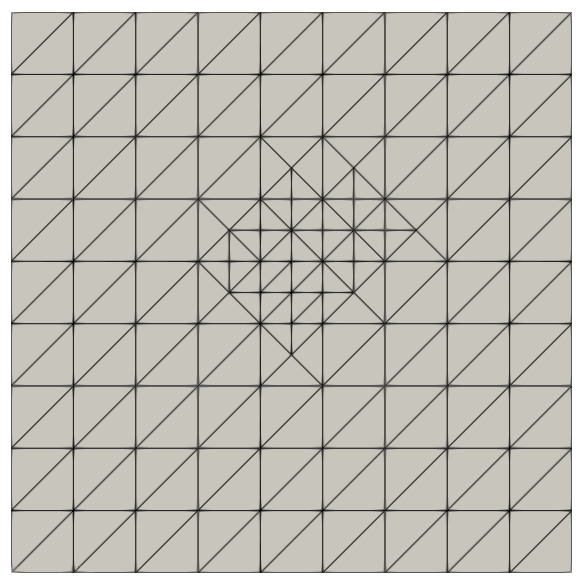
\includegraphics[width=0.17\linewidth]{images/newlines/mesh/explications/addnet/refined_addnet.png}
    \end{center}

    \vspace{-10pt}
    $\cdots\longrightarrow
    \textcolor{red}{\text{INTERPOLATE}}\longrightarrow\hspace{6pt}
    \text{ESTIMATE}\hspace{8pt}\longrightarrow\hspace{14pt}
    \text{MARK}\hspace{14pt}\longrightarrow\hspace{8pt}
    \text{REFINE}\hspace{4pt}\longrightarrow\hspace{1pt}
    \cdots$

    \hspace{55pt}$\textcolor{red}{u_\theta}\hspace{55pt}\eta_{res,T}$

    \vspace{8pt}
    \textbf{Local residual estimator (in $L^2$ norm):} Let $T$ be a cell of $\mathcal{T}_h$ .

    \vspace{-8pt}
    % $$\eta_{res,T}^2 = h_T^4 \|\textcolor{red}{(\Delta u_\theta)_h + f_h}\|_{L^2(T)}^2$$
    $$\eta_{res,T}^2 = h_T^2 \|\textcolor{red}{(\Delta u_\theta)_h + f_h}\|_{L^2(T)}^2$$
    with $h_\bullet$ the size of $\bullet$ and considering the Poisson problem.
\end{frame}

\begin{frame}{Numerical results}
    \vspace{-10pt}
    \begin{center}
        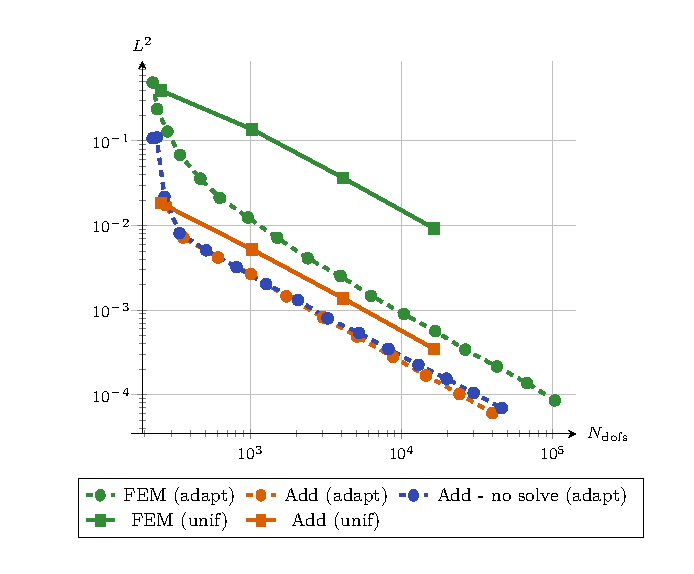
\includegraphics[width=0.4\linewidth]{images/newlines/mesh/results/cvg.pdf}
        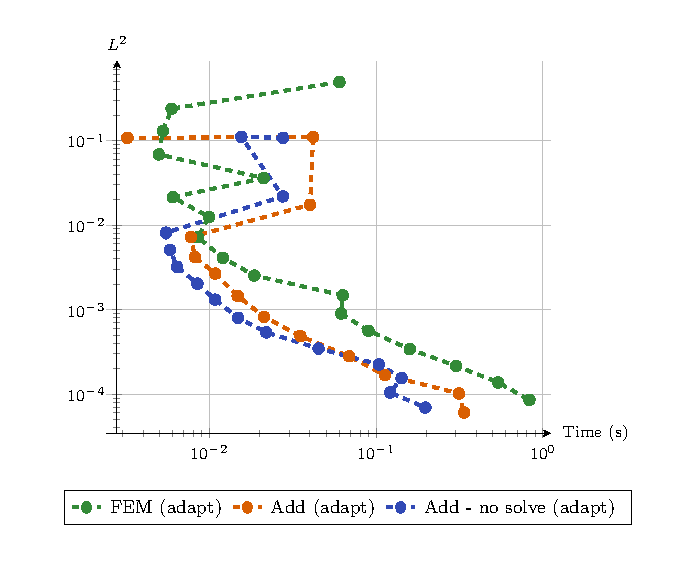
\includegraphics[width=0.4\linewidth]{images/newlines/mesh/results/times.pdf}
    \end{center}
    
    \vspace{-10pt}
    \footnotesize
    \warning \quad Results obtained on a laptop GPU (Time measurements polluted by external factors).
    
    \normalsize
    \vspace{5pt}
    \textbf{Ideas for improving results :} Additive approach (no resolution).

    \vspace{3pt}
    \begin{minipage}{0.1\linewidth}
        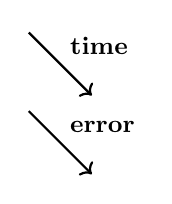
\begin{tikzpicture}[scale=1]
            \draw[->, thick] (0,1.8) -- (0.8,1);
            \node[above right] at (0.4,1.4) {\textbf{time}};

            \draw[->, thick] (0,0.8) -- (0.8,0);
            \node[above right] at (0.4,0.4) {\textbf{error}};
        \end{tikzpicture}
    \end{minipage} \hspace{5pt}
    \begin{minipage}{0.86\linewidth}
        \vspace{2pt}
        Interpolate only mesh points added in the refinement process. \\

        \vspace{5pt}
        Use another metric such as curvature, rather than residual error.

        % \vspace{-5pt}
        % $$\Delta u_\theta+f \qquad \ne \qquad u-u_\theta$$
    \end{minipage}
    % \begin{itemize}
    %     \item To improve execution times: \\ 
    %     Interpolate only mesh points added in the refinement process.
    %     % \item Cout du passage sur GPU.
    %     \item To improve the mesh : \\
    %     Use another metric such as curvature, rather than residual error. \\
    %     (The network residual ($\Delta u_\theta+f$) does not match the additive solution (the network error $u-u_\theta$).)

    % \end{itemize}

\end{frame}

\subsection{\filledstar Non linear PDEs}

\begin{frame}{Problem considered}	
    \textbf{Objective:} Extend the additive approach to non linear PDEs.

    \vspace{10pt}
    \textbf{Problem statement:} Considering the \textcolor{red}{non linear Poisson problem with Dirichlet BC}:
    \vspace{-5pt}
    \begin{equation*}
        \left\{
        \begin{aligned}
            -\text{div}\big((1+4u^4)\nabla u\big) & = f, \; &  & \text{in } \; \Omega, \\
            u         & = 1, \;  &  & \text{on } \; \partial\Omega.
        \end{aligned}
        \right.
    \end{equation*}

    with $\Omega=[-0.5\pi,0.5\pi]^2$ and $\mathcal{M}=[-0.5,0.5]^2$ ($p=2$).

    \vspace{5pt}
	\textbf{Analytical solution :}

	\vspace{-12pt}
	\begin{equation*}
		u(\bm{x};\bm{\mu})= 1 + \exp\left(-\frac{(x-\mu_1)^2+(y-\mu_2)^2}{2}\right)\sin(2x)\sin(2y)
	\end{equation*}
	\vspace{-5pt}
	
    \vspace{5pt}
	\textbf{PINN training:} Imposing BC exactly with a level-set function.

\end{frame}

\begin{frame}{Newton method}
    

    We want to solve the non linear system: \hfill \tiny $N_h$ : number of degrees of freedom.

    \normalsize
    \vspace{-10pt}
    \begin{equation}
        \label{eq:nonlinear}
        F(u) = 0 
    \end{equation}

    \vspace{-2pt}
    with $F:\mathbb{R}^{N_h} \to \mathbb{R}^{N_h}$ a non linear operator and $u\in\mathbb{R}^{N_h}$ the unknown vector.

    \begin{center}
        \small
        \begin{minipage}{0.9\linewidth}
            \begin{algorithm}[H]
                \SetAlgoLined
                \caption{Newton's method to solve \eqref{eq:nonlinear} \citep{newton_accel_2025}}
                \textbf{Initialization step:} set $u^{(0)} = u_0$\;
                \For{\( k \ge 0 \)}{
                    Solve the linear system \( F(u^{(k)}) + F'(u^{(k)}) \delta^{(k+1)} = 0 \) for \( \delta^{(k+1)} \)\;
                    Update \( u^{(k+1)} = u^{(k)} + \delta^{(k+1)} \)\;
                }
            \end{algorithm}
        \end{minipage}
    \end{center}

    \vspace{5pt}
    \textbf{Standard version:} \\
    Initialization with a constant value $u_0$. For instance, $u_0=1$.

    \vspace{5pt}
    \textbf{DeepPhysics version:} \citep{odot_deepphysics_2021} \\
    Initialization with a PINN solution $u_0=u_\theta$.
\end{frame}

\begin{frame}[noframenumbering]{Newton method}
    \vspace{5pt}
    We want to solve the non linear system: \hfill \tiny $N_h$ : number of degrees of freedom.

    \normalsize
    \vspace{-10pt}
    \begin{equation}
        F(\textcolor{red}{p_+ + u_\theta}) = 0 \tag{1}
    \end{equation}

    \vspace{-2pt}
    with $F:\mathbb{R}^{N_h} \to \mathbb{R}^{N_h}$ a non linear operator and $\textcolor{red}{p_+}\in\mathbb{R}^{N_h}$ the unknown vector.

    \begin{center}
        \small
        \begin{minipage}{0.9\linewidth}
            \begin{algorithm}[H]
                \SetAlgoLined
                \caption{\textcolor{red}{Additive approach} to solve \eqref{eq:nonlinear} }
                \textbf{Initialization step:} set \textcolor{red}{$p_+^{(0)} = 0$}\;
                \For{\( k \ge 0 \)}{
                    Solve the linear system \( F(\textcolor{red}{p_+^{(k)}+u_\theta}) + F'(\textcolor{red}{p_+^{(k)}+u_\theta}) \delta^{(k+1)} = 0 \) for \( \delta^{(k+1)} \)\;
                    Update \( \textcolor{red}{p_+^{(k+1)}} = \textcolor{red}{p_+^{(k)}} + \delta^{(k+1)} \)\;
                }
            \end{algorithm}
        \end{minipage}
    \end{center}

    \textbf{Advantage compared to DeepPhysics:}

    \begin{center}
    $u_\theta$ is not required to live in the same space as $p_+$.
    \end{center}
\end{frame}

\begin{frame}{Numerical results}	
    \vspace{-10pt}
    \begin{center}
        \begin{minipage}{0.54\linewidth}
            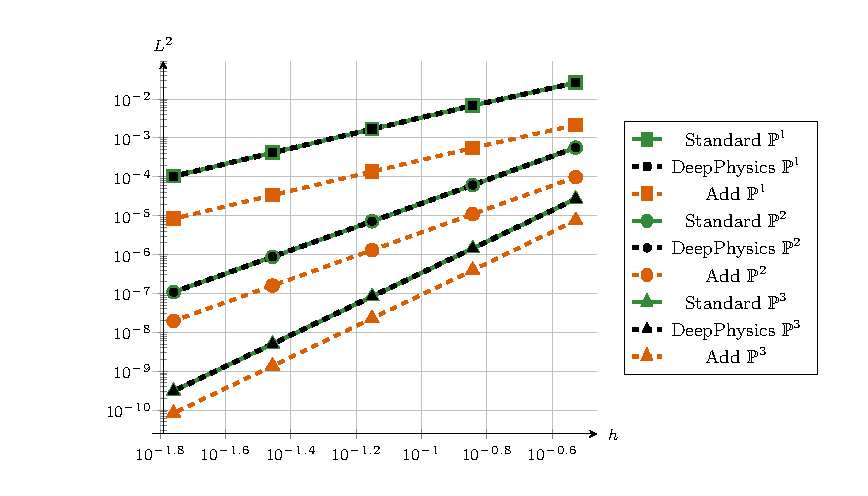
\includegraphics[width=\linewidth]{images/newlines/nonlinear/results/cvg_cropped.pdf}
        \end{minipage}
        \begin{minipage}{0.42\linewidth}
            \small
            \textbf{Number of iterations :}

            \begin{itemize}
                \item Standard Newton: $8$ iterations.
                \item DeepPhysics: $4$ iterations.
                \item Additive approach: $4$ iterations.
            \end{itemize}
        \end{minipage}
        
        \vspace{-6pt}
        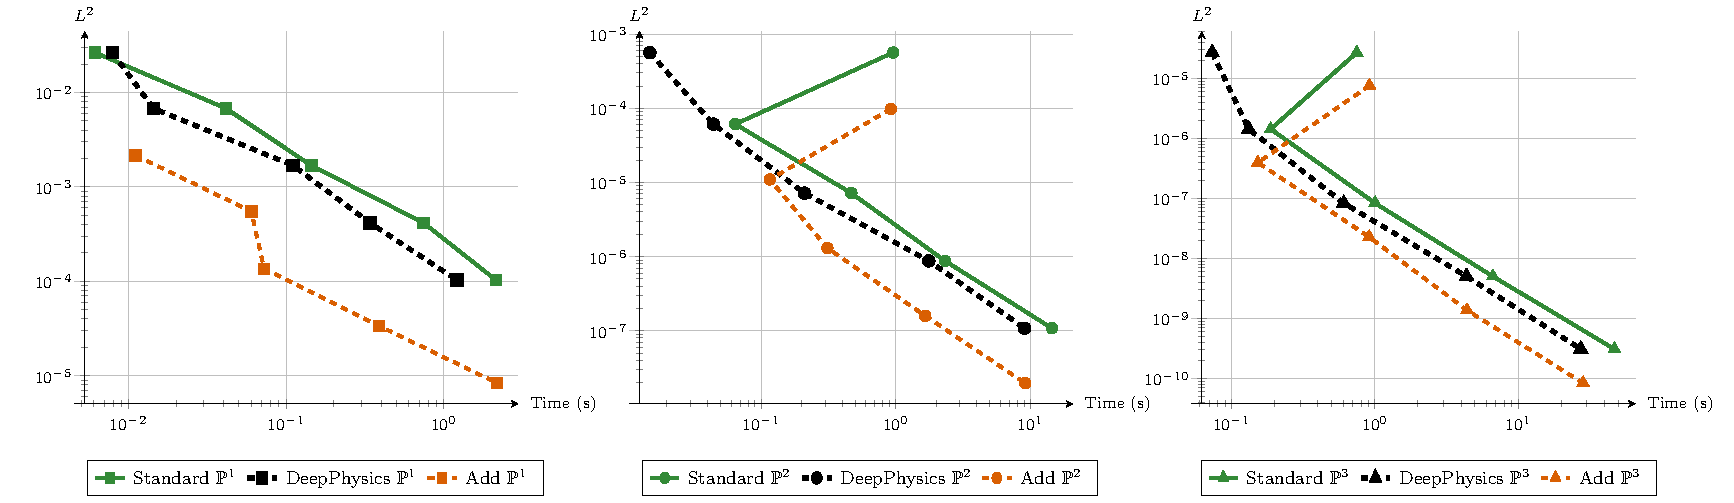
\includegraphics[width=\linewidth]{images/newlines/nonlinear/results/times.pdf}
    \end{center}
\end{frame}

	\section{Supplementary work}
	\begin{frame}{Supplementary work I}
	\small
	\vspace{-10pt}
	\begin{tcolorbox}[
		skin=bicolor,
		colback=other, % Couleur de fond de la boîte
		colbacklower=other!20!white,
		title={Teaching},
		colframe=title, % Couleur du cadre de la boîte
		arc=2mm, % Rayon de l'arrondi des coins
		boxrule=0.5pt, % Épaisseur du cadre de la boîte
		breakable, enhanced jigsaw,
		width=\linewidth,
		opacityback=0.1,
		]

		\begin{itemize}[\textcolor{other}{$\blacktriangleright$}]
			\item 2024/2025 :
			\begin{itemize}[\textcolor{other}{$\blacktriangleright$}]
                \item $64$h of Computer Science Practical Work - L1S2 and L2S3 (Python) / L3S6 (C++)
                \item $3$ days supervising a group of high school girls in RJMI \\
                ("Rendez-vous des Jeunes Mathématiciennes et Informaticiennes")
            \end{itemize}
            \item 2023/2024 : $50$h of Computer Science Practical Work - L2S3 (Python) / L3S6 (C++)
		\end{itemize}
	\end{tcolorbox}

    \vspace{-7pt}
	\begin{tcolorbox}[
		skin=bicolor,
		colback=other, % Couleur de fond de la boîte
		colbacklower=other!20!white,
		title={Training courses (Total : $176$h$35$)},
		colframe=title, % Couleur du cadre de la boîte
		arc=2mm, % Rayon de l'arrondi des coins
		boxrule=0.5pt, % Épaisseur du cadre de la boîte
		breakable, enhanced jigsaw,
		width=\linewidth,
		opacityback=0.1
		]
		
		\begin{itemize}[\textcolor{other}{$\blacktriangleright$}]
			\item A dozen seminars organized by IRMA ($\approx 10h$)
            \item 1 Deep Learning introductory course - FIDLE ($\approx 40h$)
            \item 2 workshops on Scientific Machine Learning ($\approx 2\times 21h$)
            \item 1 summer school on "New Trend in computing" ($\approx 27h$)
            \item several cross-disciplinary courses - Methodology, scientific English, etc. ($\approx 58h$)
		\end{itemize} 
	\end{tcolorbox}
\end{frame}

\begin{frame}{Supplementary work II}
    \small 

	\begin{tcolorbox}[
		skin=bicolor,
		colback=other, % Couleur de fond de la boîte
		colbacklower=other!20!white,
		title={Talks},
		%		colframe=white, % Couleur du cadre de la boîte
		arc=2mm, % Rayon de l'arrondi des coins
		boxrule=0.5pt, % Épaisseur du cadre de la boîte
		breakable, enhanced jigsaw,
		width=\linewidth,
		opacityback=0.1
		]
		
		\begin{itemize}[\textcolor{other}{$\blacktriangleright$}]
            \item \textbf{\href{https://icosahom2025.org/}{ICOSAHOM 2025}, Montréal} - July 2025 \textit{(Coming soon...)} \\
            "Enriching continuous Lagrange finite element approximation spaces using neural networks" 
            \item \textbf{\href{https://dte_aicomas_2025.iacm.info/organizers}{DTE \& AICOMAS 2025}, Paris} - February 20, 2025 \\
            \href{https://flecourtier.github.io/these2023/these2023/1.0.3/_attachments/presentation/2025_02_20.pdf}{"Combining Finite Element Methods and Neural Networks to Solve Elliptic Problems on 2D Geometries"}
			\item \textbf{Exama project, WP2 reunion} - March 26, 2024 \\
			\href{https://flecourtier.github.io/these2023/these2023/1.0.3/_attachments/presentation/2024_03_26.pdf}{"How to work with complex geometries in PINNs ?"}
			\item \textbf{Retreat (Macaron/Tonus)} - February 6, 2024 \\
			\href{https://flecourtier.github.io/these2023/these2023/1.0.3/_attachments/presentation/2024_02_06.pdf}{"Mesh-based methods and physically informed learning"}
			\item \textbf{Team meeting (Mimesis)} - December 12, 2023 \\
            \href{https://flecourtier.github.io/these2023/these2023/1.0.3/_attachments/presentation/2023_12_12.pdf}{"Development of hybrid finite element/neural network methods to help create digital surgical twins"}
		\end{itemize}
	\end{tcolorbox}
\end{frame}

\begin{frame}{Supplementary work III}
    \small
	% \vspace{-7pt}
	\begin{tcolorbox}[
		skin=bicolor,
		colback=other, % Couleur de fond de la boîte
		colbacklower=other!20!white,
		title={Posters},
		%		colframe=white, % Couleur du cadre de la boîte
		arc=2mm, % Rayon de l'arrondi des coins
		boxrule=0.5pt, % Épaisseur du cadre de la boîte
		breakable, enhanced jigsaw,
		width=\linewidth,
		opacityback=0.1
		]
		
        \begin{itemize}[\textcolor{other}{$\blacktriangleright$}]
            \item \textbf{\href{https://www.mate.polimi.it/events/EMS-TAG-SciML-25/index.php}{EMS-TAG-SciML 2025}, Milan} - March 24, 2025 - \href{https://flecourtier.github.io/these2023/these2023/1.0.3/_attachments/poster/2025_03_24.pdf}{"Enriching continuous Lagrange finite element approximation spaces using neural networks"} 
            \item \textbf{\href{https://cjc-ma2024.sciencesconf.org/program?lang=fr}{CJC-MA 2024}, Lyon} - October 29, 2024 - \href{https://flecourtier.github.io/these2023/these2023/1.0.3/_attachments/poster/2024_10_24.pdf}{"Combining Finite Element Methods and Neural Networks to Solve Elliptic Problems on 2D Geometries"}
            \item \textbf{MSII poster day, Strasbourg} - October 24, 2024 \\
			\item \textbf{\href{https://irma.math.unistra.fr/~micheldansac/SciML2024/participants.html}{SciML 2024}, Strasbourg} - July 08, 2024 \\
		\end{itemize}
	\end{tcolorbox}

    \normalsize
    \begin{tcolorbox}[
		skin=bicolor,
		colback=other, % Couleur de fond de la boîte
		colbacklower=other!20!white,
		title={Publications},
		%		colframe=white, % Couleur du cadre de la boîte
		arc=2mm, % Rayon de l'arrondi des coins
		boxrule=0.5pt, % Épaisseur du cadre de la boîte
		breakable, enhanced jigsaw,
		width=\linewidth,
		opacityback=0.1
		]
		
		\begin{itemize}[\textcolor{other}{$\blacktriangleright$}]
			\item Enriching continuous lagrange finite element approximation spaces using neural networks. \textit{\small(submitted in February 2025, M2AN journal)} \\
			H. Barucq, M. Duprez, F. Faucher, E. Franck, \textbf{F. Lecourtier}, V. Lleras, V. Michel-Dansac, and N. Victorion.
		\end{itemize}
	\end{tcolorbox}
	
\end{frame}



	\section*{Conclusion}

	\begin{frame}{Conclusion}
		\textbf{Enriched finite element method using PINNs}
		\begin{itemize}
			\item PINNs are good candidates for the enriched approach. \refappendix{frame:datavspinns}
			\item Numerical validation of the theoretical results.
			\item The enriched approach provides the same results as the standard FEM method, but with coarser meshes.
			$\Rightarrow$ Reduction of the computational cost.
		\end{itemize}
		We have also tested a multiplicative approach. \refappendix{frame:mult}

		\vspace{10pt}
		\textbf{New lines of research}
		\begin{itemize}
			\item The treatment of complex geometries is progressing.
			\item New PDEs begin to be considered, in particular non-linear problems.
			\item Other methods for improving the additive approach are being studied, including posterior error estimators.
		\end{itemize}
	\end{frame}
	
	{\setbeamertemplate{footline}{} 	
	\begin{frame}{References}
		\tiny
		\bibliography{biblio}
	\end{frame}
	}
	\addtocounter{framenumber}{-1} 
	
	% \section{Appendix}
	
	\appendix
	
	% \section{\appendixname~\theappendixframenumber~: Data vs PINNs}\labelappendixframe{frame:fem}

\begin{frame}{\appendixname~\theappendixframenumber~: Data vs PINNs}\labelappendixframe{frame:datavspinns}
	TODO
\end{frame}
\addtocounter{appendixframenumber}{1}

% \section{\appendixname~\theappendixframenumber~: Data vs PINNs}\labelappendixframe{frame:fem}

\begin{frame}{\appendixname~\theappendixframenumber~: Multiplicative approach}\labelappendixframe{frame:mult}
	TODO
\end{frame}
\addtocounter{appendixframenumber}{1}


\begin{frame}{\appendixname~\theappendixframenumber~: Non-linear problems}\labelappendixframe{frame:nonlinear}
	TODO
\end{frame}
\addtocounter{appendixframenumber}{1}
	
\end{document}
